\subsection{Data MC comparison plots for all variables used in the analysis}


\begin{figure}[tbp]
  \begin{center}
    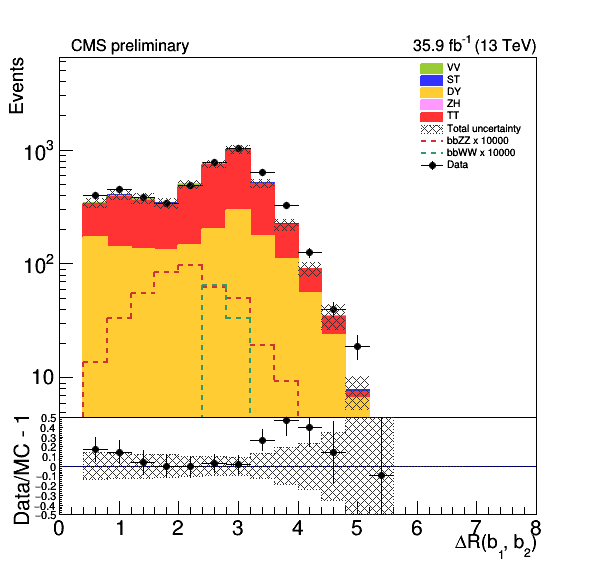
\includegraphics[width=0.31\textwidth]{figures/ee_300_april18/dR_bjets_ee_CRDY_prefit_plot_apr18.png}
    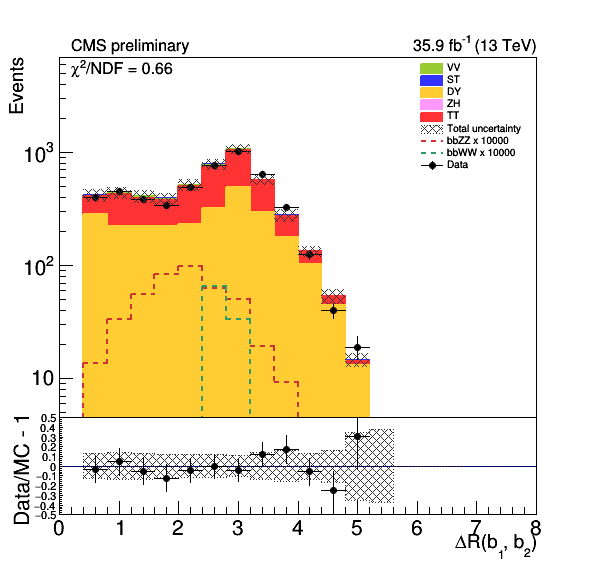
\includegraphics[width=0.31\textwidth]{figures/ee_300_april18/dR_bjets_ee_CRDY_FullPostfit_plot_apr18.png}\\
    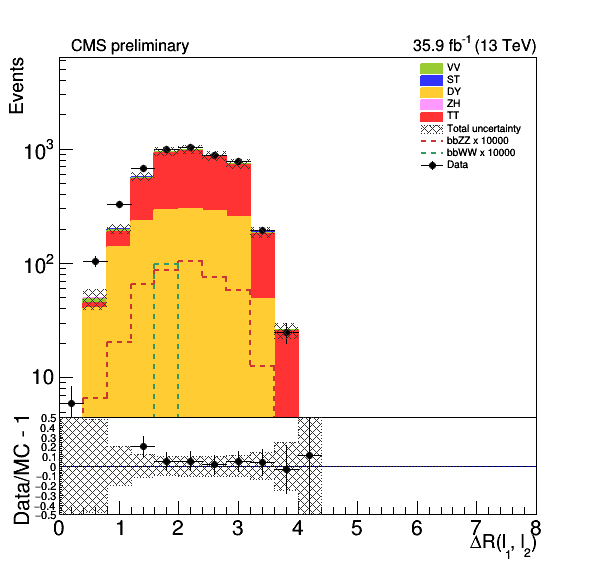
\includegraphics[width=0.31\textwidth]{figures/ee_300_april18/dR_leps_ee_CRDY_prefit_plot_apr18.png}
    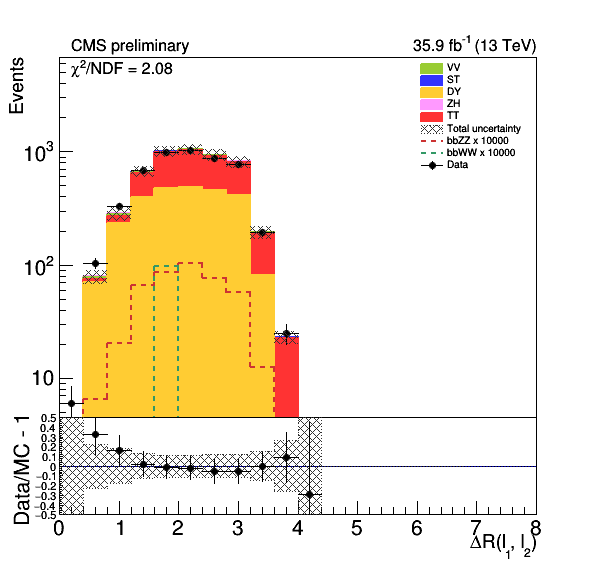
\includegraphics[width=0.31\textwidth]{figures/ee_300_april18/dR_leps_ee_CRDY_FullPostfit_plot_apr18.png}\\
    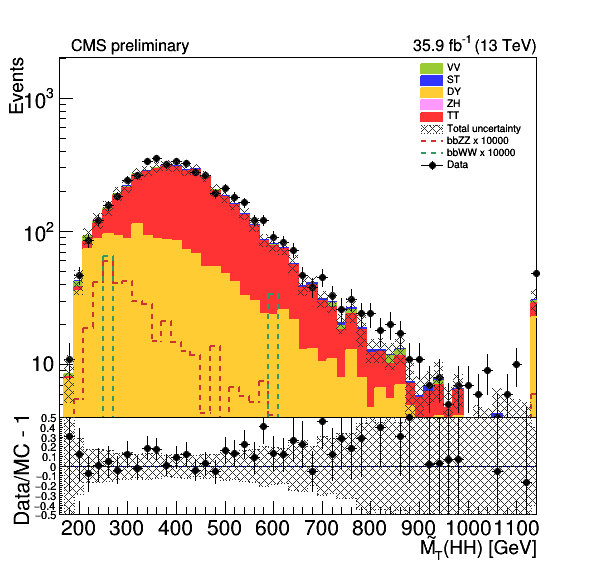
\includegraphics[width=0.31\textwidth]{figures/ee_300_april18/hhMt_ee_CRDY_prefit_plot_apr18.png}
    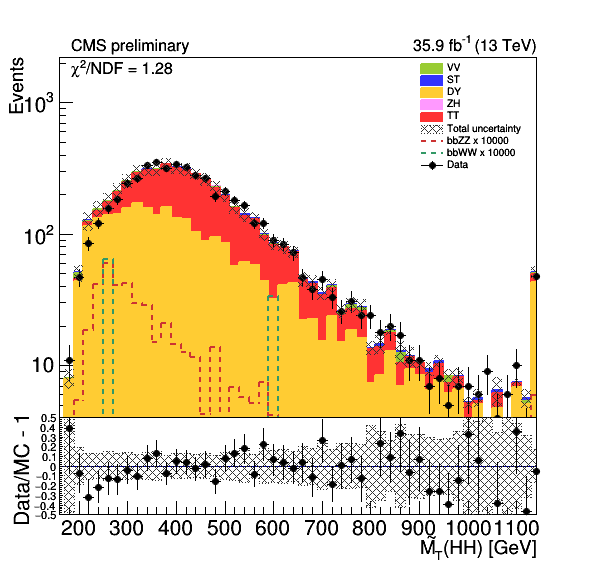
\includegraphics[width=0.31\textwidth]{figures/ee_300_april18/hhMt_ee_CRDY_FullPostfit_plot_apr18.png}\\
    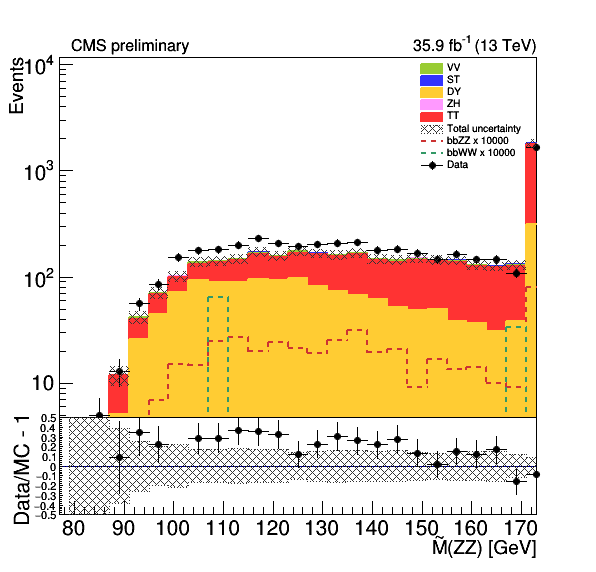
\includegraphics[width=0.31\textwidth]{figures/ee_300_april18/hmass0_ee_CRDY_prefit_plot_apr18.png}
    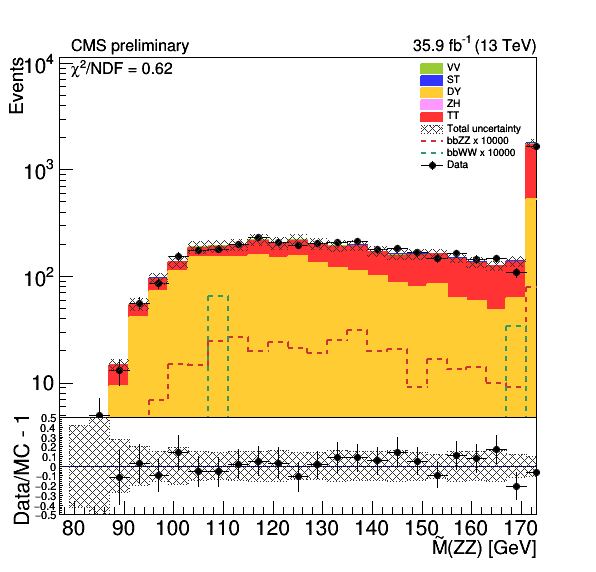
\includegraphics[width=0.31\textwidth]{figures/ee_300_april18/hmass0_ee_CRDY_FullPostfit_plot_apr18.png}\\
    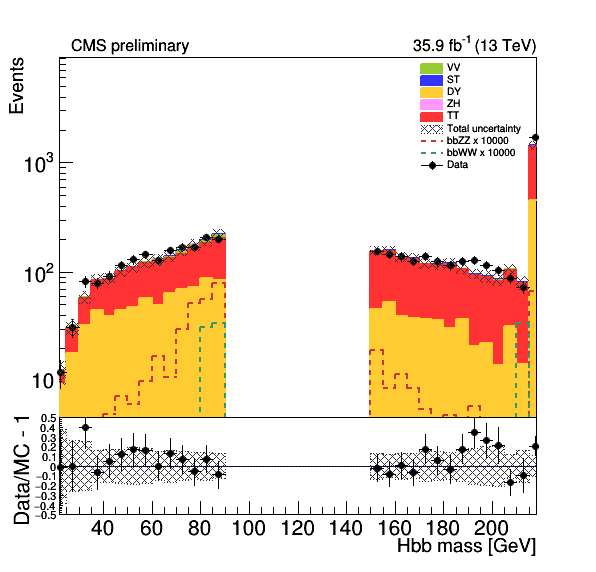
\includegraphics[width=0.31\textwidth]{figures/ee_300_april18/hmass1_ee_CRDY_prefit_plot_apr18.png}
    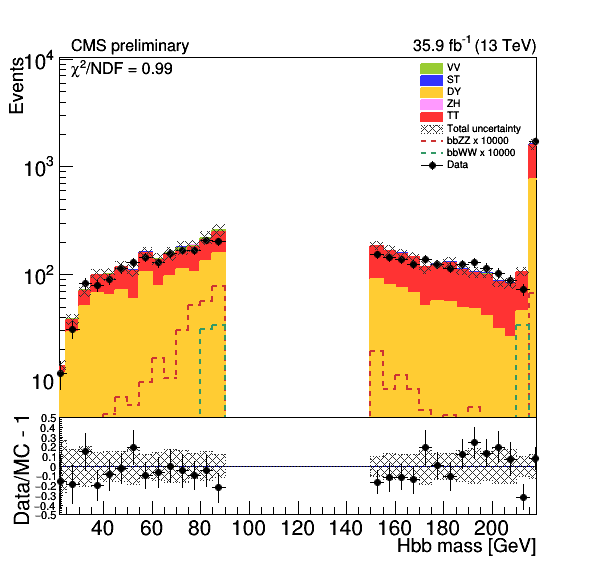
\includegraphics[width=0.31\textwidth]{figures/ee_300_april18/hmass1_ee_CRDY_FullPostfit_plot_apr18.png}\\
    \caption{Comparison of data and MC samples. 300 GeV, CRDY region, ee channel. Prefit plot on the left,           Full Postfit plot on the right.}
    \label{fig:MCcomparisons_ee_low_CRDY}
  \end{center}
\end{figure}

\begin{figure}[tbp]
  \begin{center}
    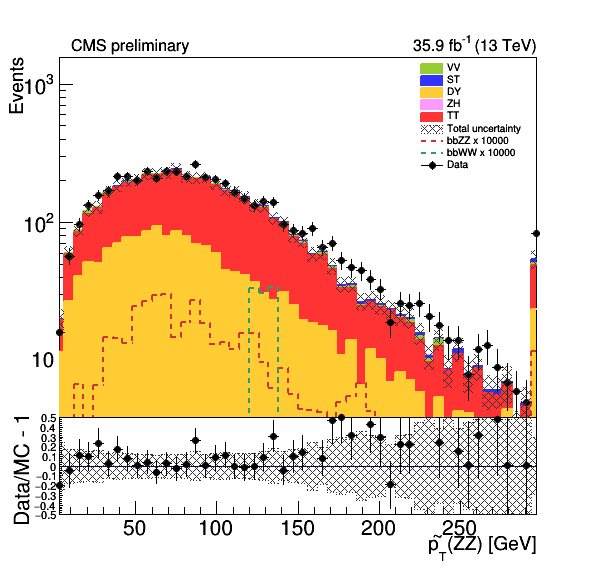
\includegraphics[width=0.31\textwidth]{figures/ee_300_april18/hpt0_ee_CRDY_prefit_plot_apr18.png}
    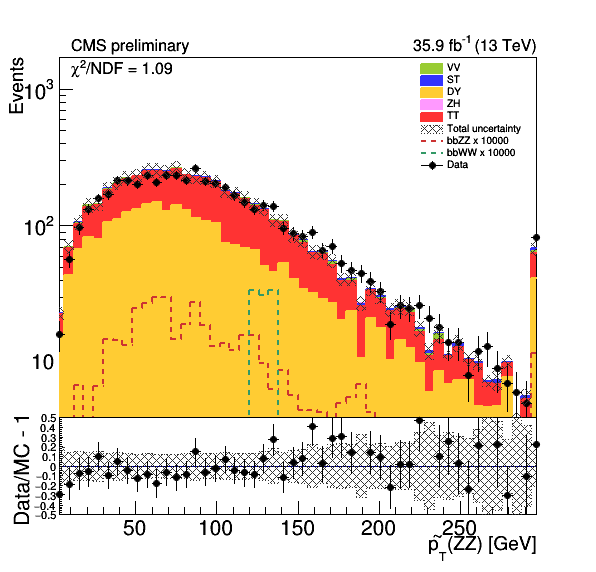
\includegraphics[width=0.31\textwidth]{figures/ee_300_april18/hpt0_ee_CRDY_FullPostfit_plot_apr18.png}\\
    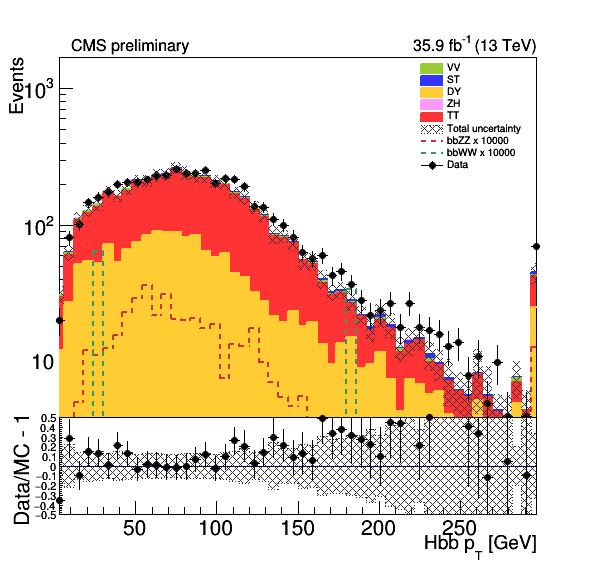
\includegraphics[width=0.31\textwidth]{figures/ee_300_april18/hpt1_ee_CRDY_prefit_plot_apr18.png}
    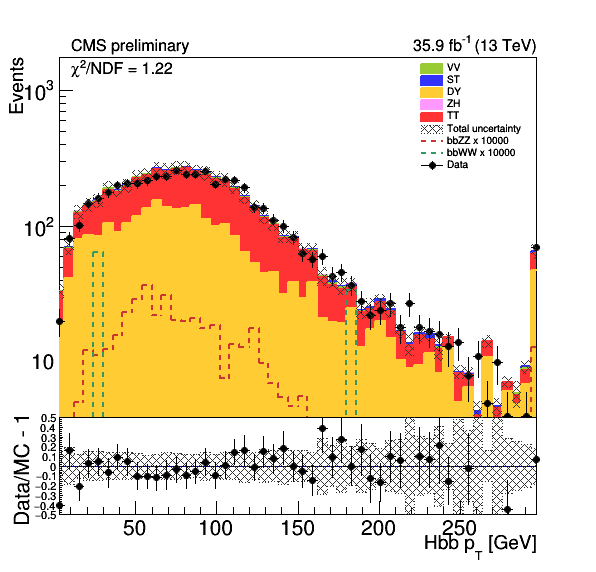
\includegraphics[width=0.31\textwidth]{figures/ee_300_april18/hpt1_ee_CRDY_FullPostfit_plot_apr18.png}\\
    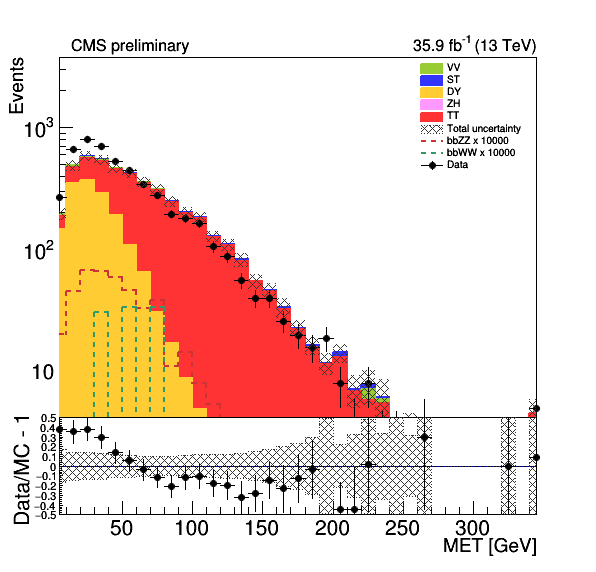
\includegraphics[width=0.31\textwidth]{figures/ee_300_april18/met_pt_ee_CRDY_prefit_plot_apr18.png}
    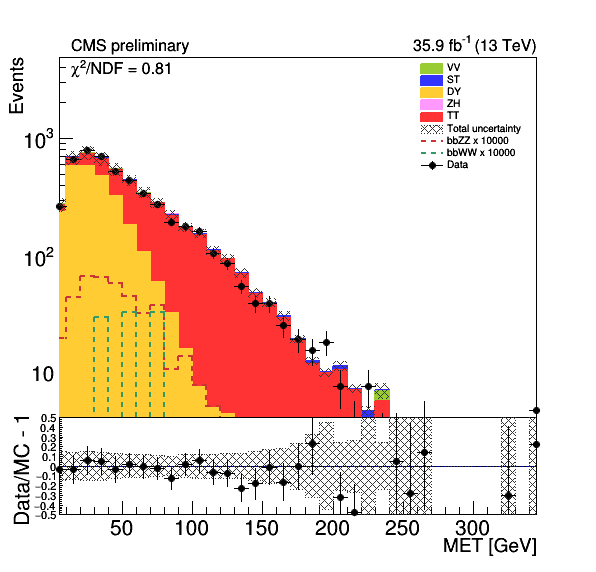
\includegraphics[width=0.31\textwidth]{figures/ee_300_april18/met_pt_ee_CRDY_FullPostfit_plot_apr18.png}\\
    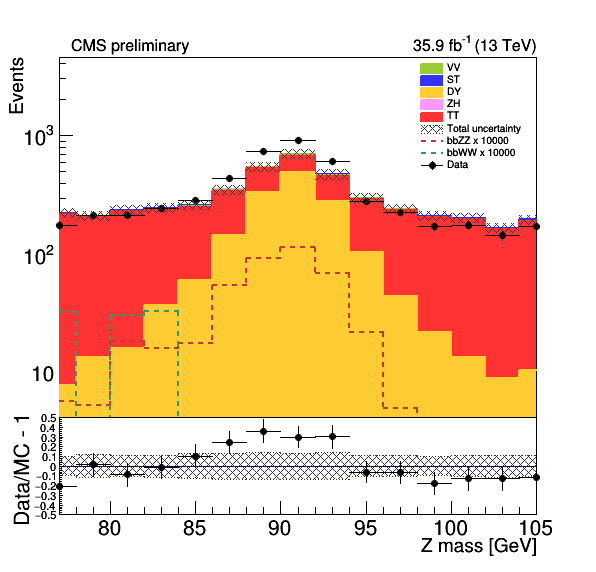
\includegraphics[width=0.31\textwidth]{figures/ee_300_april18/zmass_ee_CRDY_prefit_plot_apr21.png}
    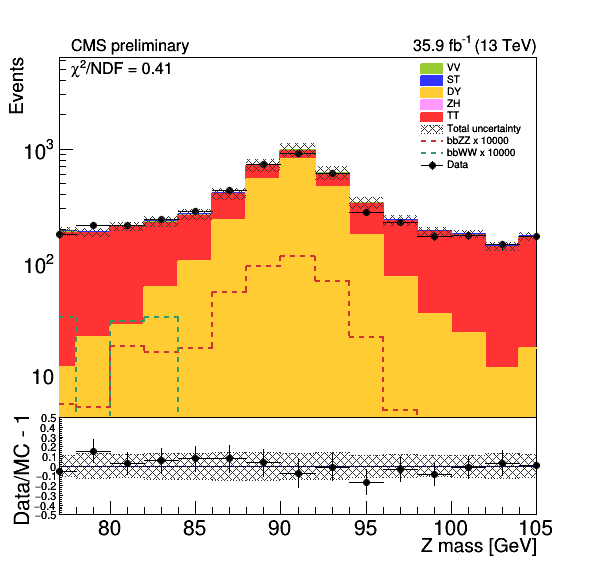
\includegraphics[width=0.31\textwidth]{figures/ee_300_april18/zmass_ee_CRDY_FullPostfit_plot_apr21.png}\\
%    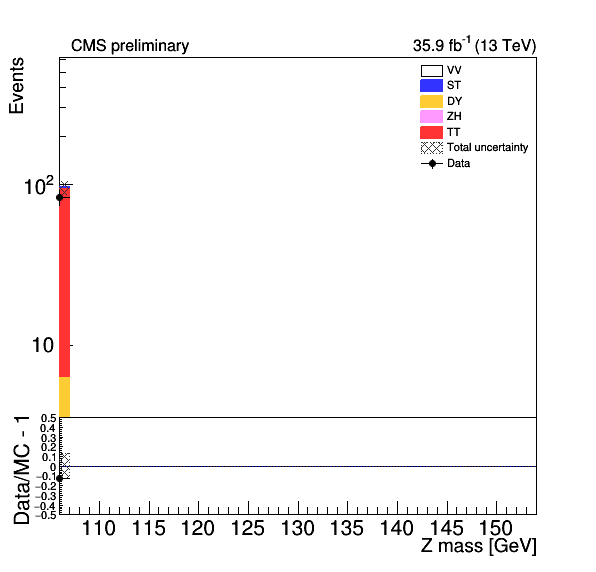
\includegraphics[width=0.31\textwidth]{figures/ee_300_april18/zmass_high_ee_CRDY_prefit_plot_apr18.png}                                                       
%    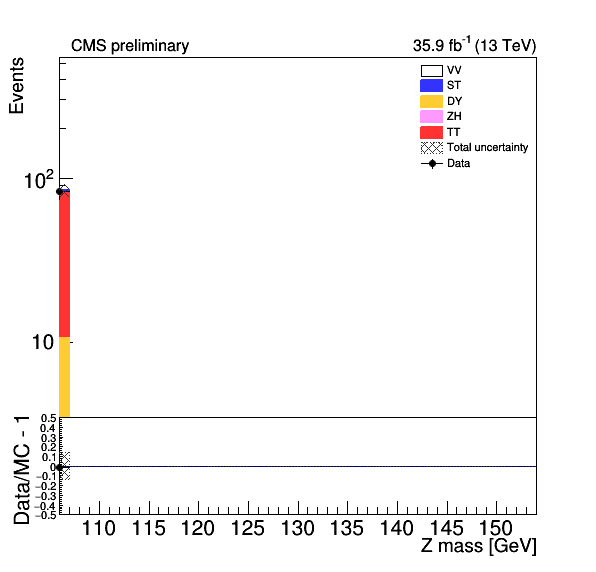
\includegraphics[width=0.31\textwidth]{figures/ee_300_april18/zmass_high_ee_CRDY_FullPostfit_plot_apr18.png}\\                                                
    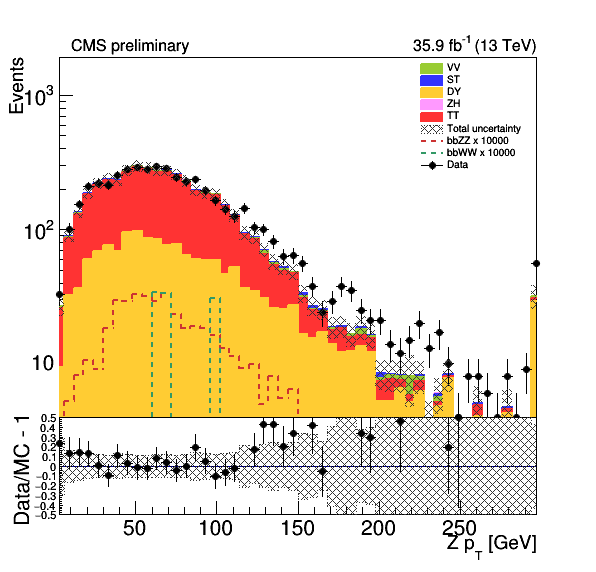
\includegraphics[width=0.31\textwidth]{figures/ee_300_april18/zpt0_ee_CRDY_prefit_plot_apr18.png}
    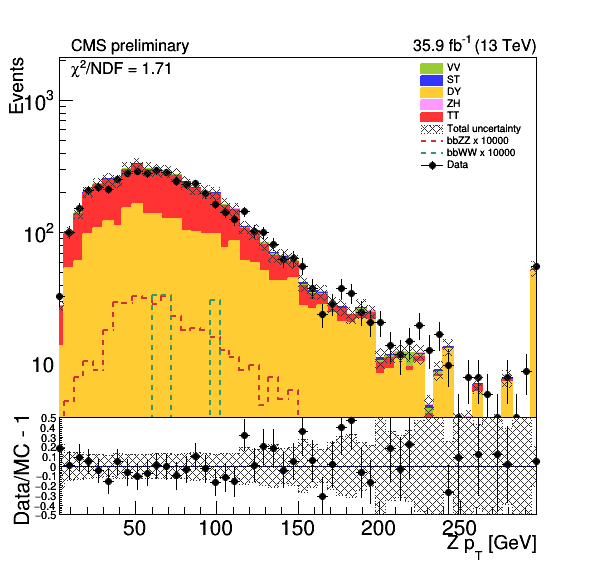
\includegraphics[width=0.31\textwidth]{figures/ee_300_april18/zpt0_ee_CRDY_FullPostfit_plot_apr18.png}\\
    \caption{Comparison of data and MC samples. 300 GeV, CRDY region, ee channel. Prefit plot on the left,           Full Postfit plot on the right.}
    \label{fig:MCcomparisons_ee_low_CRDY_2}
  \end{center}
\end{figure}


%~~~~~~~~~~~~~~~~~~~~~~~~~~~~~~~~~~~~~~~~~~~~~~~~~~~~~~~~~~~~~~~~~~~~~~~~~~~~~~~~~~~~~~~~~~~~~~~~~~~~                                                                                                             

\begin{figure}[tbp]
  \begin{center}
    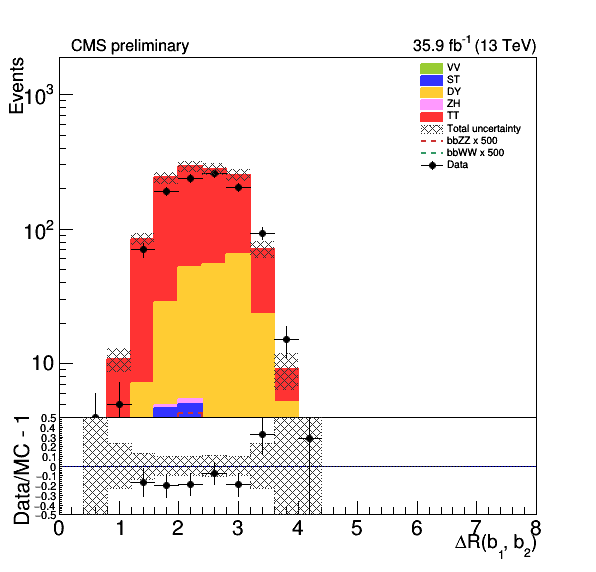
\includegraphics[width=0.31\textwidth]{figures/ee_300_april18/ee_300_good_SR_bdt_sideBand_april18/dR_bjets_ee_SR_prefit_plot_apr18.png}
    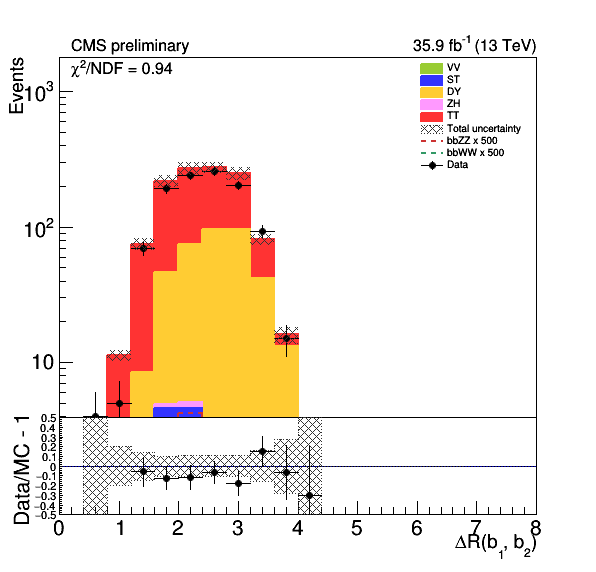
\includegraphics[width=0.31\textwidth]{figures/ee_300_april18/ee_300_good_SR_bdt_sideBand_april18/dR_bjets_ee_SR_FullPostfit_plot_apr18.png}\\
    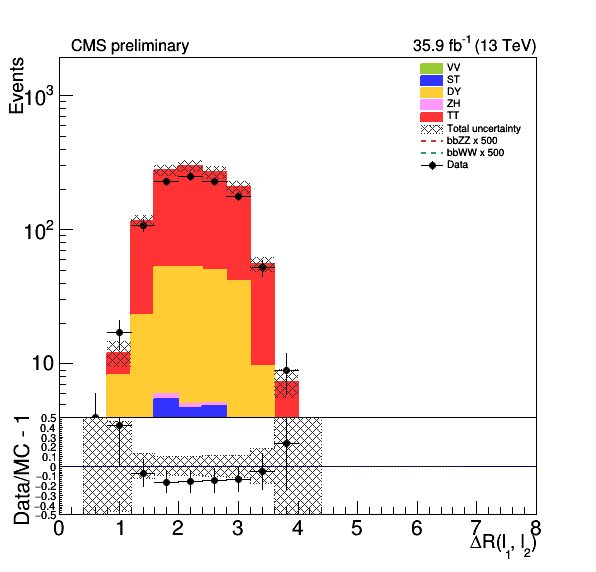
\includegraphics[width=0.31\textwidth]{figures/ee_300_april18/ee_300_good_SR_bdt_sideBand_april18/dR_leps_ee_SR_prefit_plot_apr18.png}
    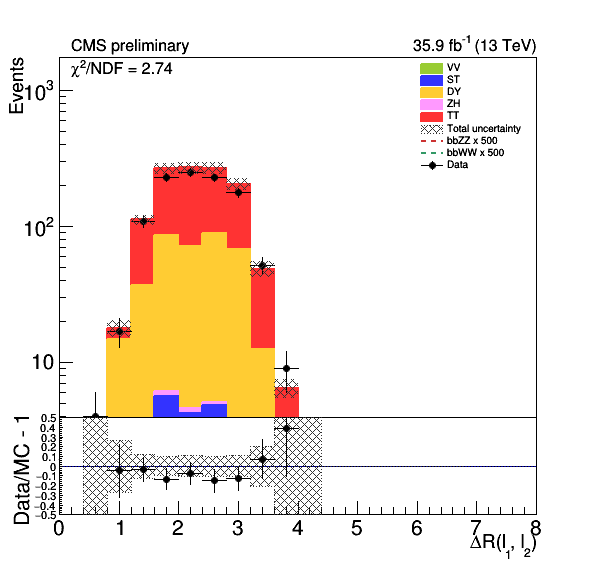
\includegraphics[width=0.31\textwidth]{figures/ee_300_april18/ee_300_good_SR_bdt_sideBand_april18/dR_leps_ee_SR_FullPostfit_plot_apr18.png}\\
    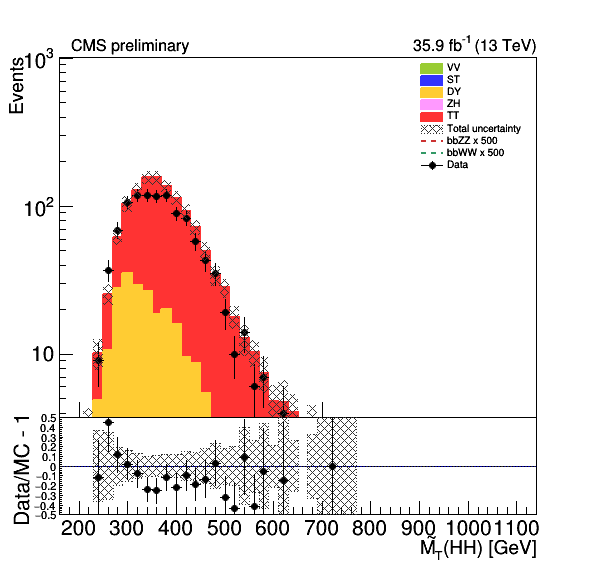
\includegraphics[width=0.31\textwidth]{figures/ee_300_april18/ee_300_good_SR_bdt_sideBand_april18/hhMt_ee_SR_prefit_plot_apr18.png}
    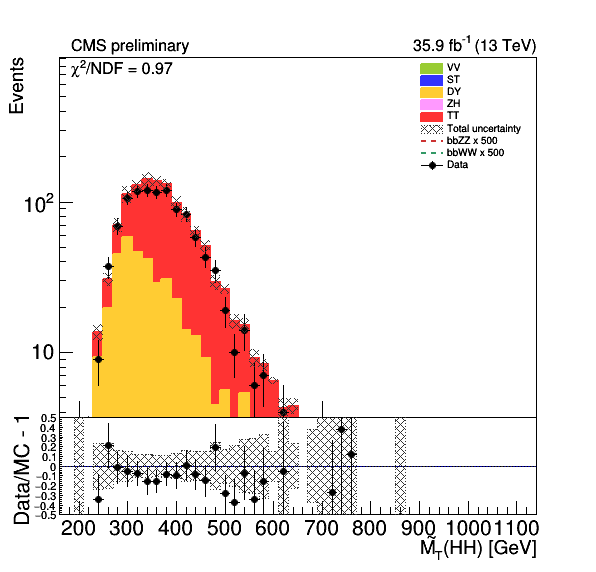
\includegraphics[width=0.31\textwidth]{figures/ee_300_april18/ee_300_good_SR_bdt_sideBand_april18/hhMt_ee_SR_FullPostfit_plot_apr18.png}\\
    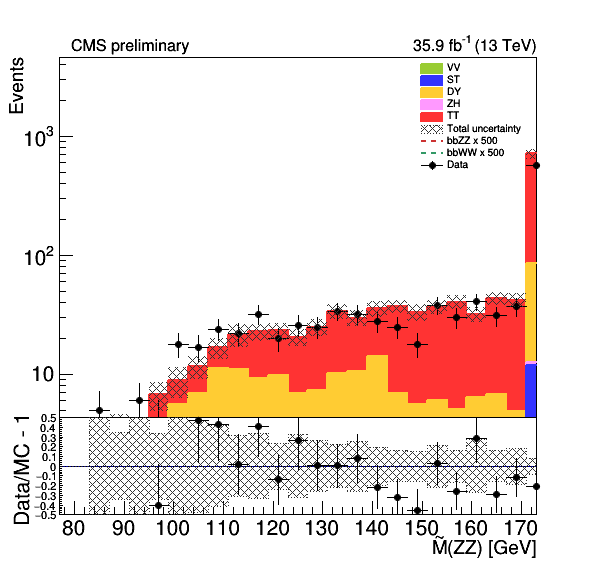
\includegraphics[width=0.31\textwidth]{figures/ee_300_april18/ee_300_good_SR_bdt_sideBand_april18/hmass0_ee_SR_prefit_plot_apr18.png}
    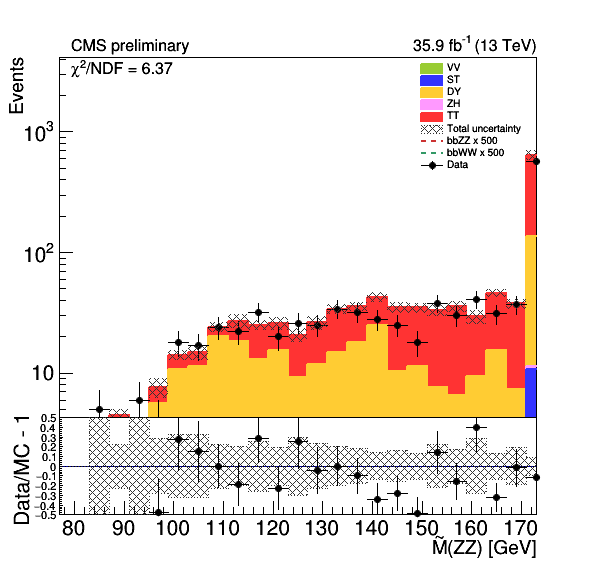
\includegraphics[width=0.31\textwidth]{figures/ee_300_april18/ee_300_good_SR_bdt_sideBand_april18/hmass0_ee_SR_FullPostfit_plot_apr18.png}\\
    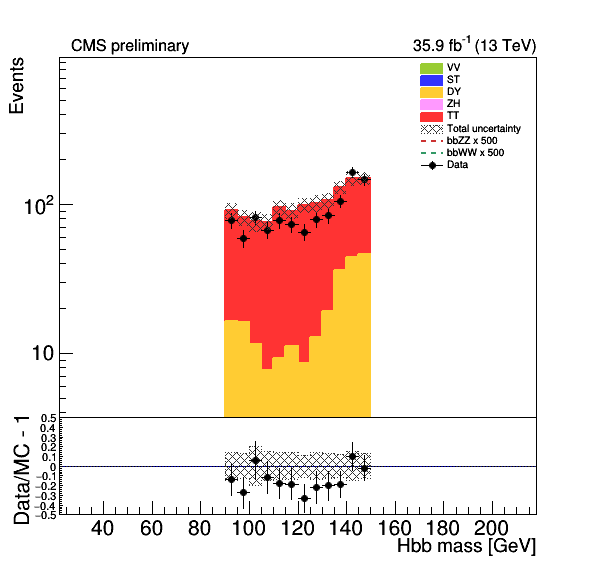
\includegraphics[width=0.31\textwidth]{figures/ee_300_april18/ee_300_good_SR_bdt_sideBand_april18/hmass1_ee_SR_prefit_plot_apr18.png}
    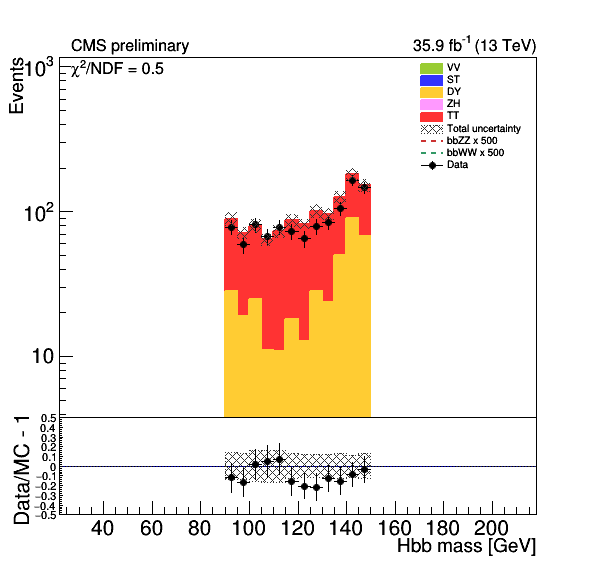
\includegraphics[width=0.31\textwidth]{figures/ee_300_april18/ee_300_good_SR_bdt_sideBand_april18/hmass1_ee_SR_FullPostfit_plot_apr18.png}\\
    \caption{Comparison of data and MC samples. 300 GeV, SR\_bdt\_sideband region, ee channel. Prefit plot on the left,           Full Postfit plot on the right. This control region was not included in the fit.}
    \label{fig:MCcomparisons_ee_low_SR_bdt_sideband}
  \end{center}
\end{figure}

\begin{figure}[tbp]
  \begin{center}
    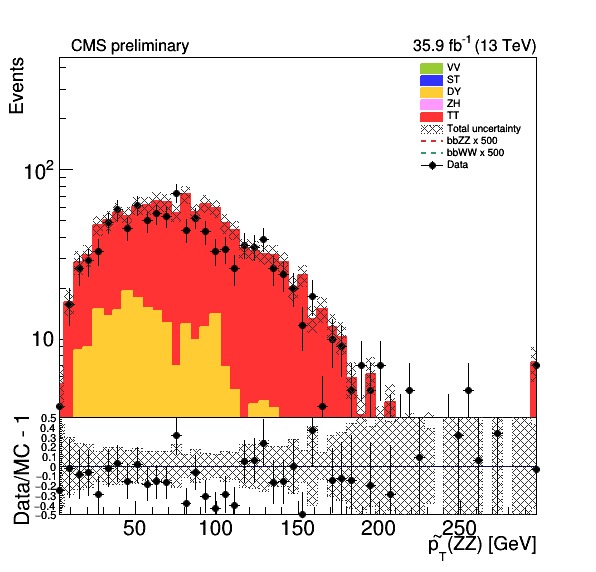
\includegraphics[width=0.31\textwidth]{figures/ee_300_april18/ee_300_good_SR_bdt_sideBand_april18/hpt0_ee_SR_prefit_plot_apr18.png}
    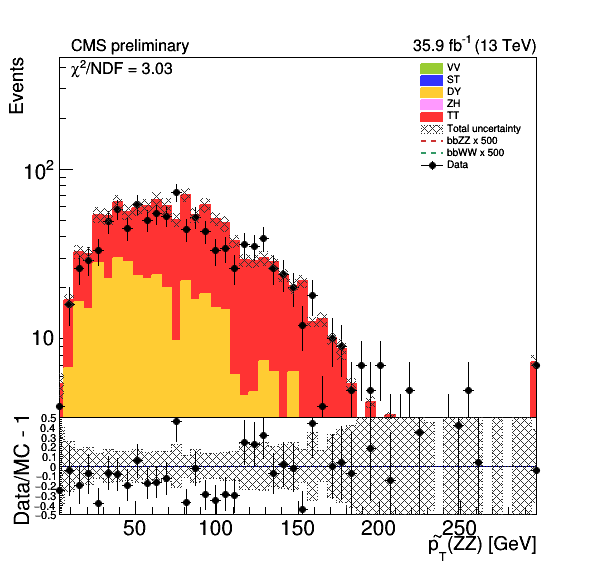
\includegraphics[width=0.31\textwidth]{figures/ee_300_april18/ee_300_good_SR_bdt_sideBand_april18/hpt0_ee_SR_FullPostfit_plot_apr18.png}\\
    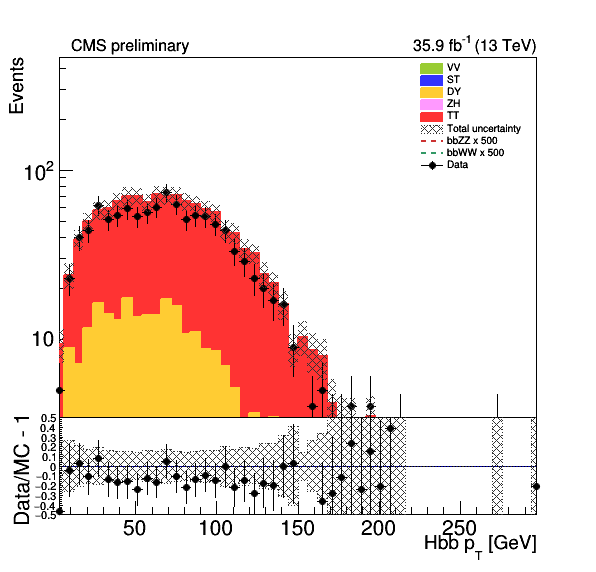
\includegraphics[width=0.31\textwidth]{figures/ee_300_april18/ee_300_good_SR_bdt_sideBand_april18/hpt1_ee_SR_prefit_plot_apr18.png}
    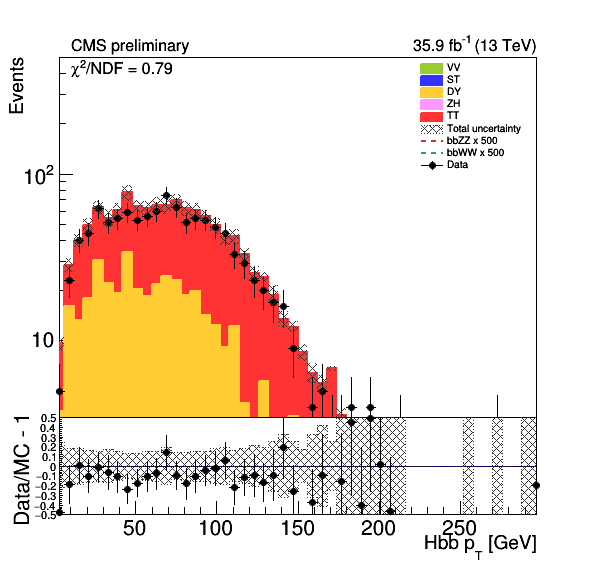
\includegraphics[width=0.31\textwidth]{figures/ee_300_april18/ee_300_good_SR_bdt_sideBand_april18/hpt1_ee_SR_FullPostfit_plot_apr18.png}\\
    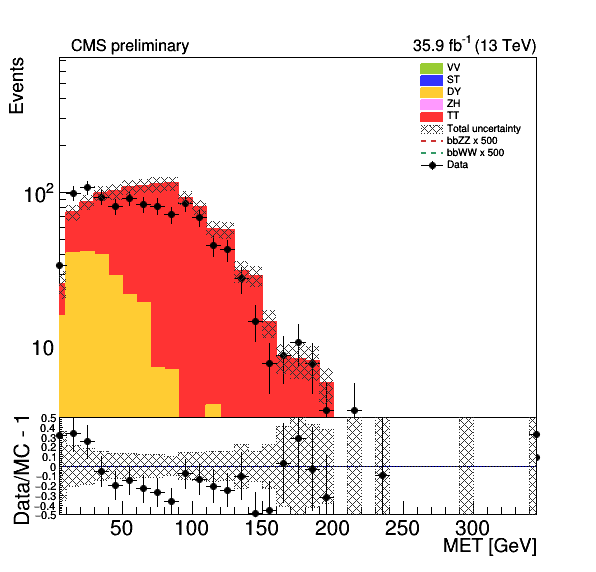
\includegraphics[width=0.31\textwidth]{figures/ee_300_april18/ee_300_good_SR_bdt_sideBand_april18/met_pt_ee_SR_prefit_plot_apr18.png}
    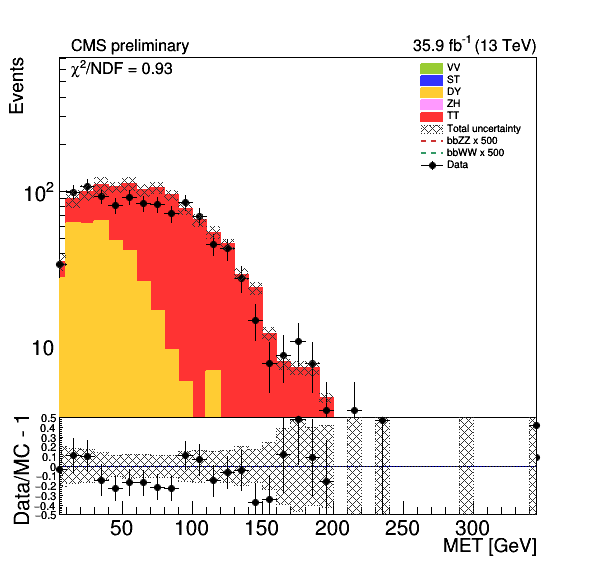
\includegraphics[width=0.31\textwidth]{figures/ee_300_april18/ee_300_good_SR_bdt_sideBand_april18/met_pt_ee_SR_FullPostfit_plot_apr18.png}\\
    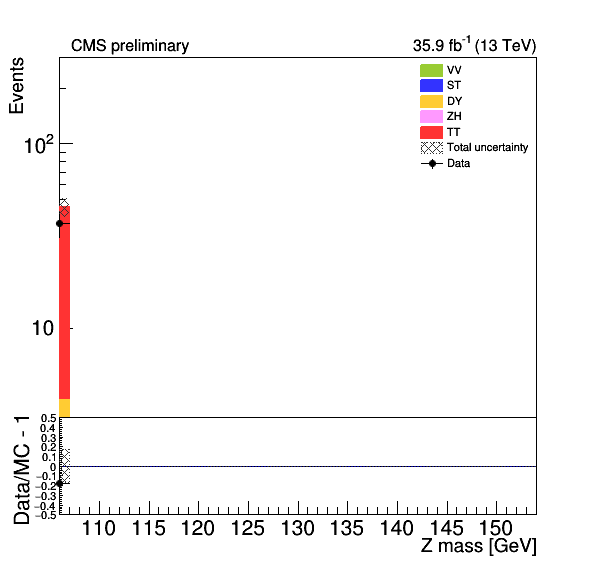
\includegraphics[width=0.31\textwidth]{figures/ee_300_april18/ee_300_good_SR_bdt_sideBand_april18/zmass_high_ee_SR_prefit_plot_apr18.png}
    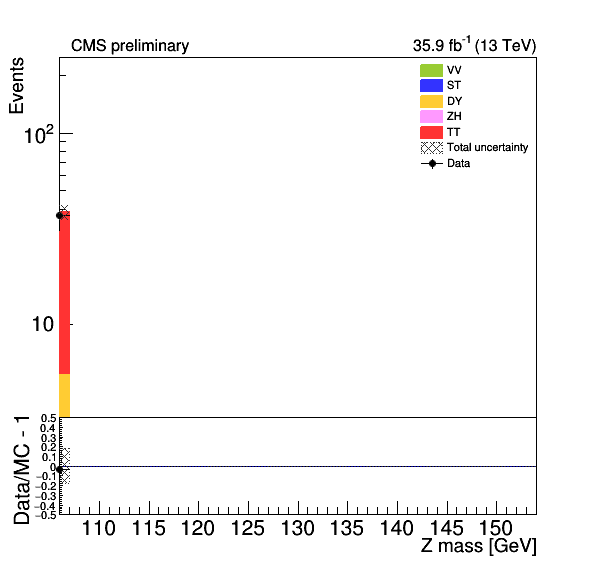
\includegraphics[width=0.31\textwidth]{figures/ee_300_april18/ee_300_good_SR_bdt_sideBand_april18/zmass_high_ee_SR_FullPostfit_plot_apr18.png}\\
    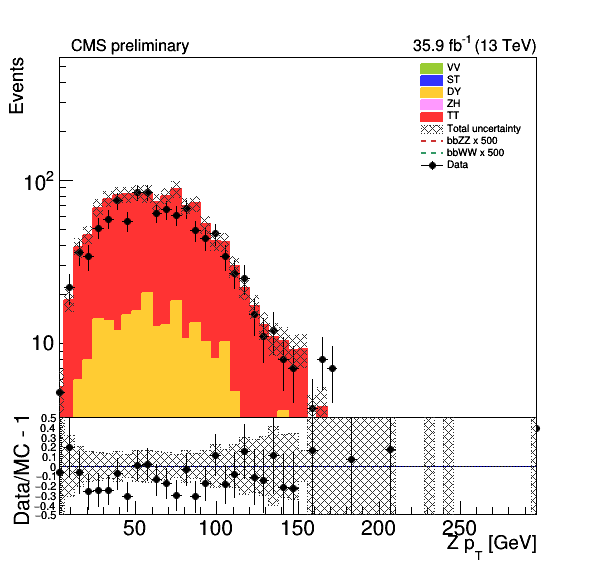
\includegraphics[width=0.31\textwidth]{figures/ee_300_april18/ee_300_good_SR_bdt_sideBand_april18/zpt0_ee_SR_prefit_plot_apr18.png}
    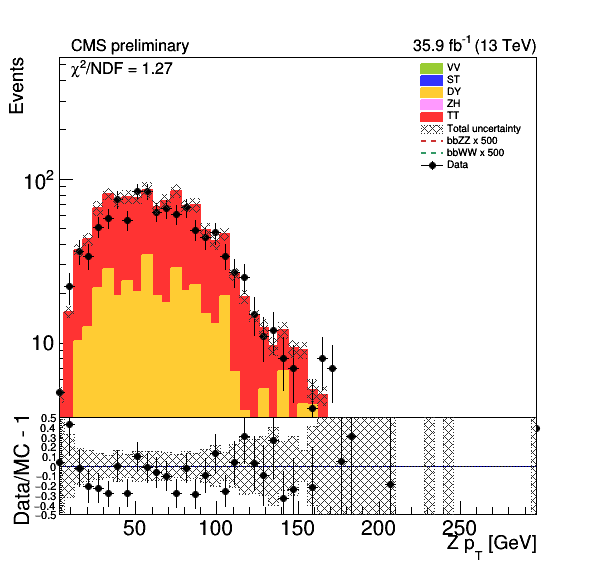
\includegraphics[width=0.31\textwidth]{figures/ee_300_april18/ee_300_good_SR_bdt_sideBand_april18/zpt0_ee_SR_FullPostfit_plot_apr18.png}\\
    \caption{Comparison of data and MC samples. 300 GeV, SR\_bdt\_sideband region, ee channel. Prefit plot on the left,           Full Postfit plot on the right. This control region was not included in the fit.}
    \label{fig:MCcomparisons_ee_low_SR_bdt_sideband_2}
  \end{center}
\end{figure}





%~~~~~~~~~~~~~~~~~~~~~~~~~~~~~~~~~~~~~~~~~~~~~~~~~~~~~~~~~~~~~~~~~~~~~~~~~~~~~~~~~~~~~~~~~~~~~~~~~~~~                                                                                                             
\begin{figure}[tbp]
  \begin{center}
    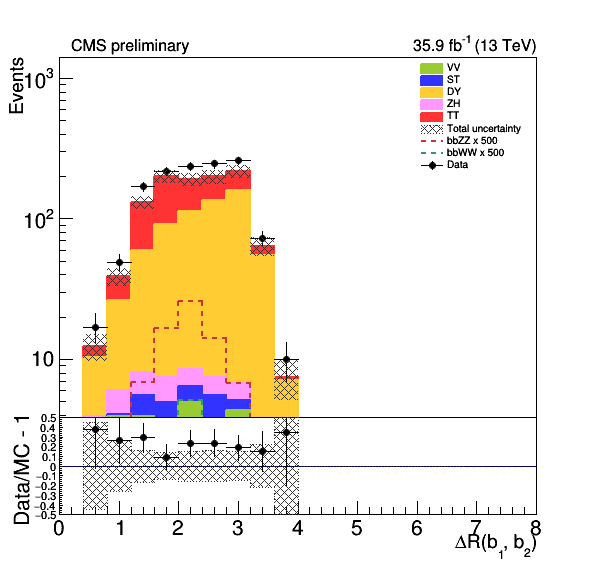
\includegraphics[width=0.31\textwidth]{figures/ee_300_SR_april21/dR_bjets_ee_SR_prefit_plot_apr21.png}
    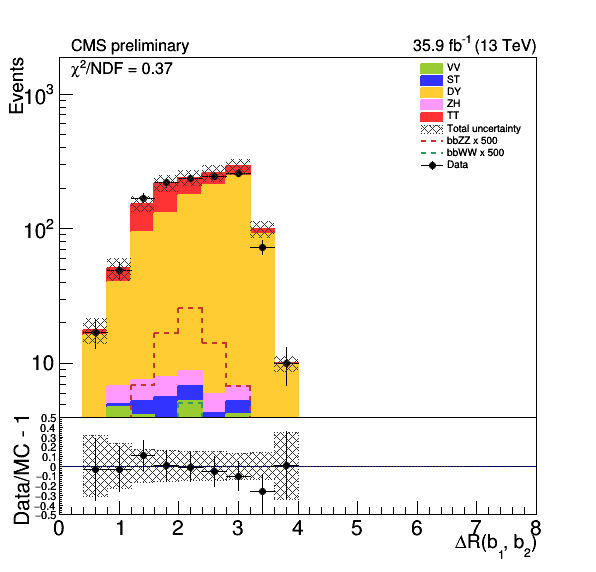
\includegraphics[width=0.31\textwidth]{figures/ee_300_SR_april21/dR_bjets_ee_SR_FullPostfit_plot_apr21.png}\\
    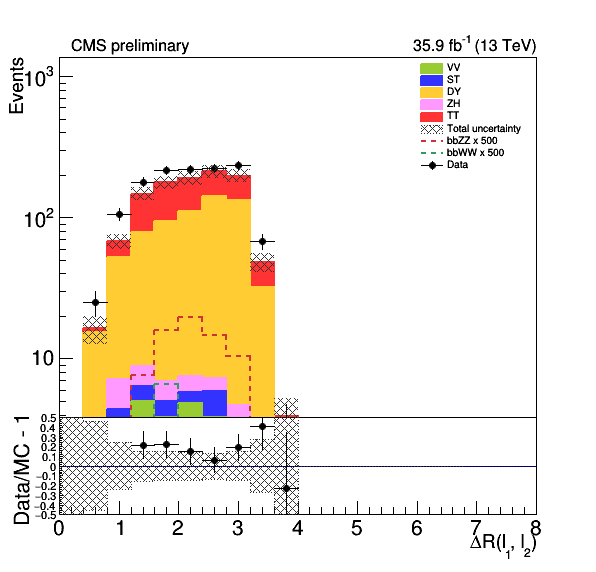
\includegraphics[width=0.31\textwidth]{figures/ee_300_SR_april21/dR_leps_ee_SR_prefit_plot_apr21.png}
    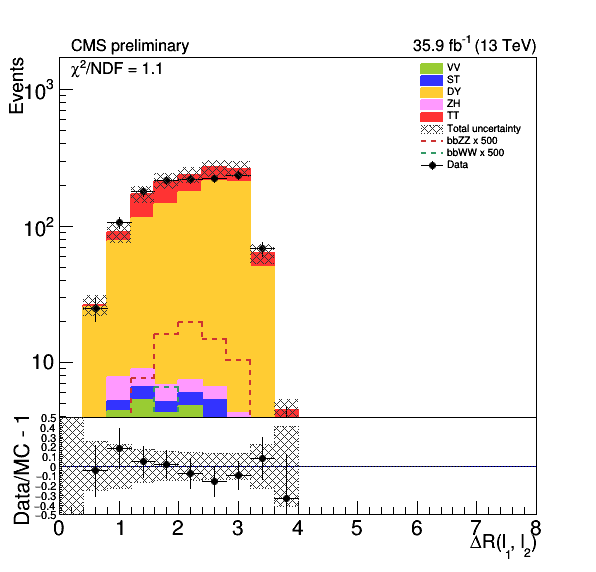
\includegraphics[width=0.31\textwidth]{figures/ee_300_SR_april21/dR_leps_ee_SR_FullPostfit_plot_apr21.png}\\
    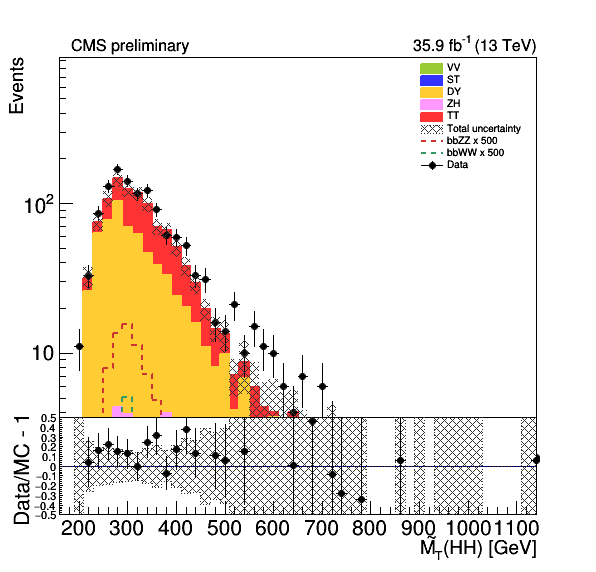
\includegraphics[width=0.31\textwidth]{figures/ee_300_SR_april21/hhMt_ee_SR_prefit_plot_apr21.png}
    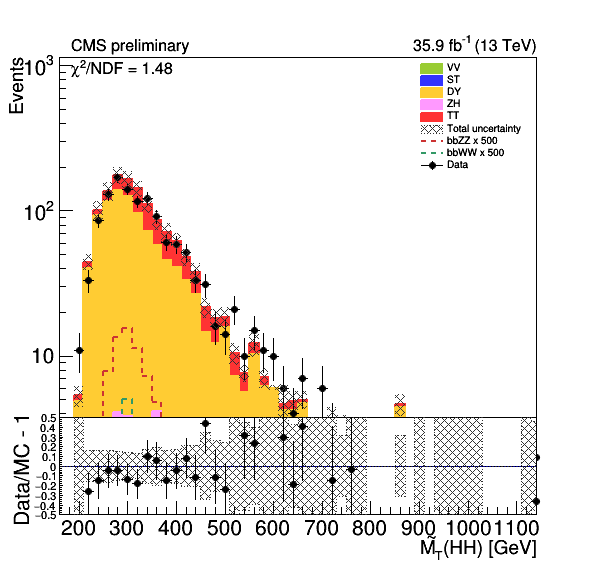
\includegraphics[width=0.31\textwidth]{figures/ee_300_SR_april21/hhMt_ee_SR_FullPostfit_plot_apr21.png}\\
    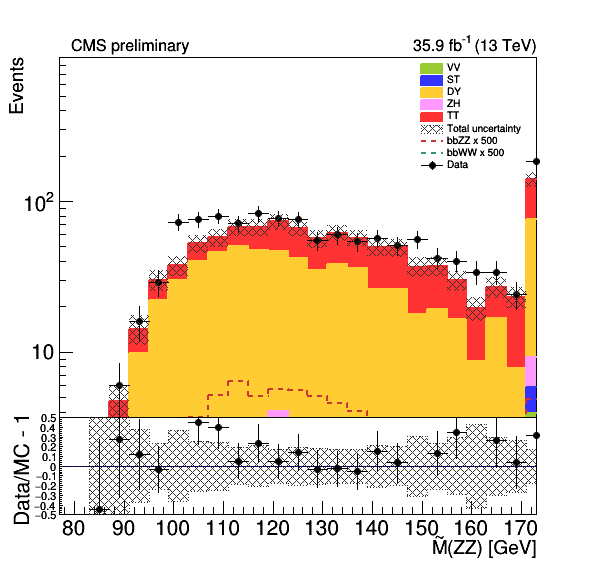
\includegraphics[width=0.31\textwidth]{figures/ee_300_SR_april21/hmass0_ee_SR_prefit_plot_apr21.png}
    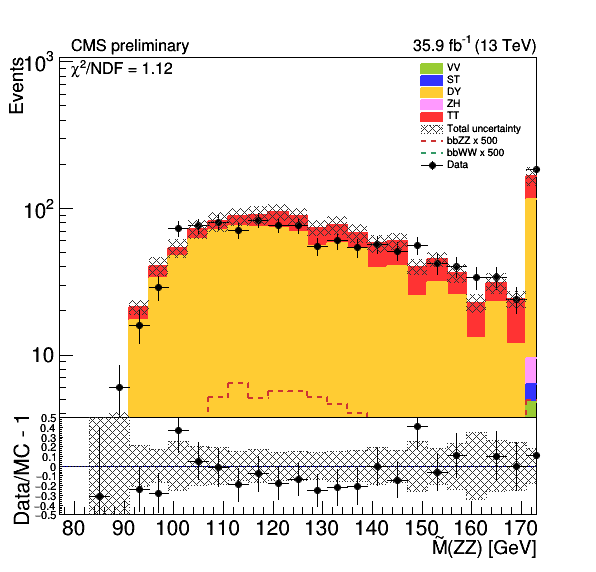
\includegraphics[width=0.31\textwidth]{figures/ee_300_SR_april21/hmass0_ee_SR_FullPostfit_plot_apr21.png}\\
    \includegraphics[width=0.31\textwidth]{figures/ee_300_SR_april21/hmass1_ee_SR_prefit_plot_apr21.png}
    \includegraphics[width=0.31\textwidth]{figures/ee_300_SR_april21/hmass1_ee_SR_FullPostfit_plot_apr21.png}\\
    \caption{Comparison of data and MC samples. 300 GeV, SR region, ee channel. Prefit plot on the left,           Full Postfit plot on the right.}
    \label{fig:MCcomparisons_ee_low_SR}
  \end{center}
\end{figure}

\begin{figure}[tbp]
  \begin{center}
    \includegraphics[width=0.31\textwidth]{figures/ee_300_SR_april21/hpt0_ee_SR_prefit_plot_apr21.png}
    \includegraphics[width=0.31\textwidth]{figures/ee_300_SR_april21/hpt0_ee_SR_FullPostfit_plot_apr21.png}\\
    \includegraphics[width=0.31\textwidth]{figures/ee_300_SR_april21/hpt1_ee_SR_prefit_plot_apr21.png}
    \includegraphics[width=0.31\textwidth]{figures/ee_300_SR_april21/hpt1_ee_SR_FullPostfit_plot_apr21.png}\\
    \includegraphics[width=0.31\textwidth]{figures/ee_300_SR_april21/met_pt_ee_SR_prefit_plot_apr21.png}
    \includegraphics[width=0.31\textwidth]{figures/ee_300_SR_april21/met_pt_ee_SR_FullPostfit_plot_apr21.png}\\
    \includegraphics[width=0.31\textwidth]{figures/ee_300_SR_april21/zmass_ee_SR_prefit_plot_apr21.png}
    \includegraphics[width=0.31\textwidth]{figures/ee_300_SR_april21/zmass_ee_SR_FullPostfit_plot_apr21.png}\\
    \includegraphics[width=0.31\textwidth]{figures/ee_300_SR_april21/zpt0_ee_SR_prefit_plot_apr21.png}
    \includegraphics[width=0.31\textwidth]{figures/ee_300_SR_april21/zpt0_ee_SR_FullPostfit_plot_apr21.png}\\
    \caption{Comparison of data and MC samples. 300 GeV, SR region, ee channel. Prefit plot on the left,           Full Postfit plot on the right.}
    \label{fig:MCcomparisons_ee_low_SR_2}
  \end{center}
\end{figure}


%~~~~~~~~~~~~~~~~~~~~~~~~~~~~~~~~~~~~~~~~~~~~~~~~~~~~~~~~~~~~~~~~~~~~~~~~~~~~~~~~~~~~~~~~~~~~~~~~~~~~                                                                                                             

\begin{figure}[tbp]
  \begin{center}
    \includegraphics[width=0.31\textwidth]{figures/ee_300_april18/dR_bjets_ee_CRTT_prefit_plot_apr18.png}
    \includegraphics[width=0.31\textwidth]{figures/ee_300_april18/dR_bjets_ee_CRTT_FullPostfit_plot_apr18.png}\\
    \includegraphics[width=0.31\textwidth]{figures/ee_300_april18/dR_leps_ee_CRTT_prefit_plot_apr18.png}
    \includegraphics[width=0.31\textwidth]{figures/ee_300_april18/dR_leps_ee_CRTT_FullPostfit_plot_apr18.png}\\
    \includegraphics[width=0.31\textwidth]{figures/ee_300_april18/hhMt_ee_CRTT_prefit_plot_apr18.png}
    \includegraphics[width=0.31\textwidth]{figures/ee_300_april18/hhMt_ee_CRTT_FullPostfit_plot_apr18.png}\\
    \includegraphics[width=0.31\textwidth]{figures/ee_300_april18/hmass0_ee_CRTT_prefit_plot_apr18.png}
    \includegraphics[width=0.31\textwidth]{figures/ee_300_april18/hmass0_ee_CRTT_FullPostfit_plot_apr18.png}\\
    \includegraphics[width=0.31\textwidth]{figures/ee_300_april18/hmass1_ee_CRTT_prefit_plot_apr18.png}
    \includegraphics[width=0.31\textwidth]{figures/ee_300_april18/hmass1_ee_CRTT_FullPostfit_plot_apr18.png}\\
    \caption{Comparison of data and MC samples. 300 GeV, CRTT region, ee channel. Prefit plot on the left,           Full Postfit plot on the right.}
    \label{fig:MCcomparisons_ee_low_CRTT}
  \end{center}
\end{figure}

\begin{figure}[tbp]
  \begin{center}
    \includegraphics[width=0.31\textwidth]{figures/ee_300_april18/hpt0_ee_CRTT_prefit_plot_apr18.png}
    \includegraphics[width=0.31\textwidth]{figures/ee_300_april18/hpt0_ee_CRTT_FullPostfit_plot_apr18.png}\\
    \includegraphics[width=0.31\textwidth]{figures/ee_300_april18/hpt1_ee_CRTT_prefit_plot_apr18.png}
    \includegraphics[width=0.31\textwidth]{figures/ee_300_april18/hpt1_ee_CRTT_FullPostfit_plot_apr18.png}\\
    \includegraphics[width=0.31\textwidth]{figures/ee_300_april18/met_pt_ee_CRTT_prefit_plot_apr18.png}
    \includegraphics[width=0.31\textwidth]{figures/ee_300_april18/met_pt_ee_CRTT_FullPostfit_plot_apr18.png}\\
    \includegraphics[width=0.31\textwidth]{figures/ee_300_april18/zmass_high_ee_CRTT_prefit_plot_apr18.png}
    \includegraphics[width=0.31\textwidth]{figures/ee_300_april18/zmass_high_ee_CRTT_FullPostfit_plot_apr18.png}\\
    \includegraphics[width=0.31\textwidth]{figures/ee_300_april18/zpt0_ee_CRTT_prefit_plot_apr18.png}
    \includegraphics[width=0.31\textwidth]{figures/ee_300_april18/zpt0_ee_CRTT_FullPostfit_plot_apr18.png}\\
    \caption{Comparison of data and MC samples. 300 GeV, CRTT region, ee channel. Prefit plot on the left,           Full Postfit plot on the right.}
    \label{fig:MCcomparisons_ee_low_CRTT_2}
  \end{center}
\end{figure}




%~~~~~~~~~~~~~~~~~~~~~~~~~~~~~~~~~~~~~~~~~~~~~~~~~~~~~~~~~~~~~~~~~~~~~~~~~~~~~~~~~~~~~~~~~~~~~~~~~~~~                                                                                                             



\begin{figure}[tbp]
  \begin{center}
    \includegraphics[width=0.31\textwidth]{figures/mm_300_april18/dR_bjets_mm_CRDY_prefit_plot_apr18.png}
    \includegraphics[width=0.31\textwidth]{figures/mm_300_april18/dR_bjets_mm_CRDY_FullPostfit_plot_apr18.png}\\
    \includegraphics[width=0.31\textwidth]{figures/mm_300_april18/dR_leps_mm_CRDY_prefit_plot_apr18.png}
    \includegraphics[width=0.31\textwidth]{figures/mm_300_april18/dR_leps_mm_CRDY_FullPostfit_plot_apr18.png}\\
    \includegraphics[width=0.31\textwidth]{figures/mm_300_april18/hhMt_mm_CRDY_prefit_plot_apr18.png}
    \includegraphics[width=0.31\textwidth]{figures/mm_300_april18/hhMt_mm_CRDY_FullPostfit_plot_apr18.png}\\
    \includegraphics[width=0.31\textwidth]{figures/mm_300_april18/hmass0_mm_CRDY_prefit_plot_apr18.png}
    \includegraphics[width=0.31\textwidth]{figures/mm_300_april18/hmass0_mm_CRDY_FullPostfit_plot_apr18.png}\\
    \includegraphics[width=0.31\textwidth]{figures/mm_300_april18/hmass1_mm_CRDY_prefit_plot_apr18.png}
    \includegraphics[width=0.31\textwidth]{figures/mm_300_april18/hmass1_mm_CRDY_FullPostfit_plot_apr18.png}\\
    \caption{Comparison of data and MC samples. 300 GeV, CRDY region, mm channel. Prefit plot on the left,           Full Postfit plot on the right.}
    \label{fig:MCcomparisons_mm_low_CRDY}
  \end{center}
\end{figure}

\begin{figure}[tbp]
  \begin{center}
    \includegraphics[width=0.31\textwidth]{figures/mm_300_april18/hpt0_mm_CRDY_prefit_plot_apr18.png}
    \includegraphics[width=0.31\textwidth]{figures/mm_300_april18/hpt0_mm_CRDY_FullPostfit_plot_apr18.png}\\
    \includegraphics[width=0.31\textwidth]{figures/mm_300_april18/hpt1_mm_CRDY_prefit_plot_apr18.png}
    \includegraphics[width=0.31\textwidth]{figures/mm_300_april18/hpt1_mm_CRDY_FullPostfit_plot_apr18.png}\\
    \includegraphics[width=0.31\textwidth]{figures/mm_300_april18/met_pt_mm_CRDY_prefit_plot_apr18.png}
    \includegraphics[width=0.31\textwidth]{figures/mm_300_april18/met_pt_mm_CRDY_FullPostfit_plot_apr18.png}\\
    \includegraphics[width=0.31\textwidth]{figures/mm_300_april18/zmass_mm_CRDY_prefit_plot_apr21.png}
    \includegraphics[width=0.31\textwidth]{figures/mm_300_april18/zmass_mm_CRDY_FullPostfit_plot_apr21.png}\\
%    \includegraphics[width=0.31\textwidth]{figures/mm_300_april18/zmass_high_mm_CRDY_prefit_plot_apr18.png}                                                      
%    \includegraphics[width=0.31\textwidth]{figures/mm_300_april18/zmass_high_mm_CRDY_FullPostfit_plot_apr18.png}\\                                                 
    \includegraphics[width=0.31\textwidth]{figures/mm_300_april18/zpt0_mm_CRDY_prefit_plot_apr18.png}
    \includegraphics[width=0.31\textwidth]{figures/mm_300_april18/zpt0_mm_CRDY_FullPostfit_plot_apr18.png}\\
    \caption{Comparison of data and MC samples. 300 GeV, CRDY region, mm channel. Prefit plot on the left,           Full Postfit plot on the right.}
    \label{fig:MCcomparisons_mm_low_CRDY_2}
  \end{center}
\end{figure}





%~~~~~~~~~~~~~~~~~~~~~~~~~~~~~~~~~~~~~~~~~~~~~~~~~~~~~~~~~~~~~~~~~~~~~~~~~~~~~~~~~~~~~~~~~~~~~~~~~~~~                                                                                                             

\begin{figure}[tbp]
  \begin{center}
    \includegraphics[width=0.31\textwidth]{figures/mm_300_april18/mm_300_good_SR_bdt_sideBand_april18/dR_bjets_mm_SR_prefit_plot_apr18.png}
    \includegraphics[width=0.31\textwidth]{figures/mm_300_april18/mm_300_good_SR_bdt_sideBand_april18/dR_bjets_mm_SR_FullPostfit_plot_apr18.png}\\
    \includegraphics[width=0.31\textwidth]{figures/mm_300_april18/mm_300_good_SR_bdt_sideBand_april18/dR_leps_mm_SR_prefit_plot_apr18.png}
    \includegraphics[width=0.31\textwidth]{figures/mm_300_april18/mm_300_good_SR_bdt_sideBand_april18/dR_leps_mm_SR_FullPostfit_plot_apr18.png}\\
    \includegraphics[width=0.31\textwidth]{figures/mm_300_april18/mm_300_good_SR_bdt_sideBand_april18/hhMt_mm_SR_prefit_plot_apr18.png}
    \includegraphics[width=0.31\textwidth]{figures/mm_300_april18/mm_300_good_SR_bdt_sideBand_april18/hhMt_mm_SR_FullPostfit_plot_apr18.png}\\
    \includegraphics[width=0.31\textwidth]{figures/mm_300_april18/mm_300_good_SR_bdt_sideBand_april18/hmass0_mm_SR_prefit_plot_apr18.png}
    \includegraphics[width=0.31\textwidth]{figures/mm_300_april18/mm_300_good_SR_bdt_sideBand_april18/hmass0_mm_SR_FullPostfit_plot_apr18.png}\\
    \includegraphics[width=0.31\textwidth]{figures/mm_300_april18/mm_300_good_SR_bdt_sideBand_april18/hmass1_mm_SR_prefit_plot_apr18.png}
    \includegraphics[width=0.31\textwidth]{figures/mm_300_april18/mm_300_good_SR_bdt_sideBand_april18/hmass1_mm_SR_FullPostfit_plot_apr18.png}\\
    \caption{Comparison of data and MC samples. 300 GeV, SR\_bdt\_sideband region, mm channel. Prefit plot on the left,           Full Postfit plot on the right. This control region was not included in the fit.}
    \label{fig:MCcomparisons_mm_low_SR_bdt_sideband}
  \end{center}
\end{figure}

\begin{figure}[tbp]
  \begin{center}
    \includegraphics[width=0.31\textwidth]{figures/mm_300_april18/mm_300_good_SR_bdt_sideBand_april18/hpt0_mm_SR_prefit_plot_apr18.png}
    \includegraphics[width=0.31\textwidth]{figures/mm_300_april18/mm_300_good_SR_bdt_sideBand_april18/hpt0_mm_SR_FullPostfit_plot_apr18.png}\\
    \includegraphics[width=0.31\textwidth]{figures/mm_300_april18/mm_300_good_SR_bdt_sideBand_april18/hpt1_mm_SR_prefit_plot_apr18.png}
    \includegraphics[width=0.31\textwidth]{figures/mm_300_april18/mm_300_good_SR_bdt_sideBand_april18/hpt1_mm_SR_FullPostfit_plot_apr18.png}\\
    \includegraphics[width=0.31\textwidth]{figures/mm_300_april18/mm_300_good_SR_bdt_sideBand_april18/met_pt_mm_SR_prefit_plot_apr18.png}
    \includegraphics[width=0.31\textwidth]{figures/mm_300_april18/mm_300_good_SR_bdt_sideBand_april18/met_pt_mm_SR_FullPostfit_plot_apr18.png}\\
    \includegraphics[width=0.31\textwidth]{figures/mm_300_april18/mm_300_good_SR_bdt_sideBand_april18/zmass_high_mm_SR_prefit_plot_apr18.png}
    \includegraphics[width=0.31\textwidth]{figures/mm_300_april18/mm_300_good_SR_bdt_sideBand_april18/zmass_high_mm_SR_FullPostfit_plot_apr18.png}\\
    \includegraphics[width=0.31\textwidth]{figures/mm_300_april18/mm_300_good_SR_bdt_sideBand_april18/zpt0_mm_SR_prefit_plot_apr18.png}
    \includegraphics[width=0.31\textwidth]{figures/mm_300_april18/mm_300_good_SR_bdt_sideBand_april18/zpt0_mm_SR_FullPostfit_plot_apr18.png}\\
    \caption{Comparison of data and MC samples. 300 GeV, SR\_bdt\_sideband region, mm channel. Prefit plot on the left,           Full Postfit plot on the right. This control region was not included in the fit.}
    \label{fig:MCcomparisons_mm_low_SR_bdt_sideband_2}
  \end{center}
\end{figure}


%~~~~~~~~~~~~~~~~~~~~~~~~~~~~~~~~~~~~~~~~~~~~~~~~~~~~~~~~~~~~~~~~~~~~~~~~~~~~~~~~~~~~~~~~~~~~~~~~~~~~                                                                                                             
\begin{figure}[tbp]
  \begin{center}
    \includegraphics[width=0.31\textwidth]{figures/mm_300_SR_april21/dR_bjets_mm_SR_prefit_plot_apr21.png}
    \includegraphics[width=0.31\textwidth]{figures/mm_300_SR_april21/dR_bjets_mm_SR_FullPostfit_plot_apr21.png}\\
    \includegraphics[width=0.31\textwidth]{figures/mm_300_SR_april21/dR_leps_mm_SR_prefit_plot_apr21.png}
    \includegraphics[width=0.31\textwidth]{figures/mm_300_SR_april21/dR_leps_mm_SR_FullPostfit_plot_apr21.png}\\
    \includegraphics[width=0.31\textwidth]{figures/mm_300_SR_april21/hhMt_mm_SR_prefit_plot_apr21.png}
    \includegraphics[width=0.31\textwidth]{figures/mm_300_SR_april21/hhMt_mm_SR_FullPostfit_plot_apr21.png}\\
    \includegraphics[width=0.31\textwidth]{figures/mm_300_SR_april21/hmass0_mm_SR_prefit_plot_apr21.png}
    \includegraphics[width=0.31\textwidth]{figures/mm_300_SR_april21/hmass0_mm_SR_FullPostfit_plot_apr21.png}\\
    \includegraphics[width=0.31\textwidth]{figures/mm_300_SR_april21/hmass1_mm_SR_prefit_plot_apr21.png}
    \includegraphics[width=0.31\textwidth]{figures/mm_300_SR_april21/hmass1_mm_SR_FullPostfit_plot_apr21.png}\\
    \caption{Comparison of data and MC samples. 300 GeV, SR region, mm channel. Prefit plot on the left,           Full Postfit plot on the right.}
    \label{fig:MCcomparisons_mm_low_SR}
  \end{center}
\end{figure}

\begin{figure}[tbp]
  \begin{center}
    \includegraphics[width=0.31\textwidth]{figures/mm_300_SR_april21/hpt0_mm_SR_prefit_plot_apr21.png}
    \includegraphics[width=0.31\textwidth]{figures/mm_300_SR_april21/hpt0_mm_SR_FullPostfit_plot_apr21.png}\\
    \includegraphics[width=0.31\textwidth]{figures/mm_300_SR_april21/hpt1_mm_SR_prefit_plot_apr21.png}
    \includegraphics[width=0.31\textwidth]{figures/mm_300_SR_april21/hpt1_mm_SR_FullPostfit_plot_apr21.png}\\
    \includegraphics[width=0.31\textwidth]{figures/mm_300_SR_april21/met_pt_mm_SR_prefit_plot_apr21.png}
    \includegraphics[width=0.31\textwidth]{figures/mm_300_SR_april21/met_pt_mm_SR_FullPostfit_plot_apr21.png}\\
    \includegraphics[width=0.31\textwidth]{figures/mm_300_SR_april21/zmass_mm_SR_prefit_plot_apr21.png}
    \includegraphics[width=0.31\textwidth]{figures/mm_300_SR_april21/zmass_mm_SR_FullPostfit_plot_apr21.png}\\
    \includegraphics[width=0.31\textwidth]{figures/mm_300_SR_april21/zpt0_mm_SR_prefit_plot_apr21.png}
    \includegraphics[width=0.31\textwidth]{figures/mm_300_SR_april21/zpt0_mm_SR_FullPostfit_plot_apr21.png}\\
    \caption{Comparison of data and MC samples. 300 GeV, SR region, mm channel. Prefit plot on the left,           Full Postfit plot on the right.}
    \label{fig:MCcomparisons_mm_low_SR_2}
  \end{center}
\end{figure}





%~~~~~~~~~~~~~~~~~~~~~~~~~~~~~~~~~~~~~~~~~~~~~~~~~~~~~~~~~~~~~~~~~~~~~~~~~~~~~~~~~~~~~~~~~~~~~~~~~~~~                                                                                                             

\begin{figure}[tbp]
  \begin{center}
    \includegraphics[width=0.31\textwidth]{figures/mm_300_april18/dR_bjets_mm_CRTT_prefit_plot_apr18.png}
    \includegraphics[width=0.31\textwidth]{figures/mm_300_april18/dR_bjets_mm_CRTT_FullPostfit_plot_apr18.png}\\
    \includegraphics[width=0.31\textwidth]{figures/mm_300_april18/dR_leps_mm_CRTT_prefit_plot_apr18.png}
    \includegraphics[width=0.31\textwidth]{figures/mm_300_april18/dR_leps_mm_CRTT_FullPostfit_plot_apr18.png}\\
    \includegraphics[width=0.31\textwidth]{figures/mm_300_april18/hhMt_mm_CRTT_prefit_plot_apr18.png}
    \includegraphics[width=0.31\textwidth]{figures/mm_300_april18/hhMt_mm_CRTT_FullPostfit_plot_apr18.png}\\
    \includegraphics[width=0.31\textwidth]{figures/mm_300_april18/hmass0_mm_CRTT_prefit_plot_apr18.png}
    \includegraphics[width=0.31\textwidth]{figures/mm_300_april18/hmass0_mm_CRTT_FullPostfit_plot_apr18.png}\\
    \includegraphics[width=0.31\textwidth]{figures/mm_300_april18/hmass1_mm_CRTT_prefit_plot_apr18.png}
    \includegraphics[width=0.31\textwidth]{figures/mm_300_april18/hmass1_mm_CRTT_FullPostfit_plot_apr18.png}\\
    \caption{Comparison of data and MC samples. 300 GeV, CRTT region, mm channel. Prefit plot on the left,           Full Postfit plot on the right.}
    \label{fig:MCcomparisons_mm_low_CRTT}
  \end{center}
\end{figure}

\begin{figure}[tbp]
  \begin{center}
    \includegraphics[width=0.31\textwidth]{figures/mm_300_april18/hpt0_mm_CRTT_prefit_plot_apr18.png}
    \includegraphics[width=0.31\textwidth]{figures/mm_300_april18/hpt0_mm_CRTT_FullPostfit_plot_apr18.png}\\
    \includegraphics[width=0.31\textwidth]{figures/mm_300_april18/hpt1_mm_CRTT_prefit_plot_apr18.png}
    \includegraphics[width=0.31\textwidth]{figures/mm_300_april18/hpt1_mm_CRTT_FullPostfit_plot_apr18.png}\\
    \includegraphics[width=0.31\textwidth]{figures/mm_300_april18/met_pt_mm_CRTT_prefit_plot_apr18.png}
    \includegraphics[width=0.31\textwidth]{figures/mm_300_april18/met_pt_mm_CRTT_FullPostfit_plot_apr18.png}\\
    \includegraphics[width=0.31\textwidth]{figures/mm_300_april18/zmass_high_mm_CRTT_prefit_plot_apr18.png}
    \includegraphics[width=0.31\textwidth]{figures/mm_300_april18/zmass_high_mm_CRTT_FullPostfit_plot_apr18.png}\\
    \includegraphics[width=0.31\textwidth]{figures/mm_300_april18/zpt0_mm_CRTT_prefit_plot_apr18.png}
    \includegraphics[width=0.31\textwidth]{figures/mm_300_april18/zpt0_mm_CRTT_FullPostfit_plot_apr18.png}\\
    \caption{Comparison of data and MC samples. 300 GeV, CRTT region, mm channel. Prefit plot on the left,           Full Postfit plot on the right.}
    \label{fig:MCcomparisons_mm_low_CRTT_2}
  \end{center}
\end{figure}

%% %~~~~~~~~~~~~~~~~~~~~~~~~~~~~~~~~~~~~~~~~~~~~~~~~~~~~~~~~~                                                                                                                

\begin{figure}[tbp]                                                                                                                                                       
  \begin{center}                                                                                                                                                          
    \includegraphics[width=0.31\textwidth]{figures/ee_300_april18/bdt_response_ee_CRDY_prefit_plot_apr18.png}                                                             
    \includegraphics[width=0.31\textwidth]{figures/ee_300_april18/bdt_response_ee_CRDY_FullPostfit_plot_apr18.png}\\                                                      
    \includegraphics[width=0.31\textwidth]{figures/ee_300_april18/ee_300_good_SR_bdt_sideBand_april18/bdt_response_afterCut_ee_SR_prefit_plot_apr18.png}                  
    \includegraphics[width=0.31\textwidth]{figures/ee_300_april18/ee_300_good_SR_bdt_sideBand_april18/bdt_response_afterCut_ee_SR_FullPostfit_plot_apr18.png}\\           
    \includegraphics[width=0.31\textwidth]{figures/ee_300_SR_april21/bdt_response_afterCut_ee_SR_prefit_plot_apr21.png}                                                   
    \includegraphics[width=0.31\textwidth]{figures/ee_300_SR_april21/bdt_response_afterCut_ee_SR_FullPostfit_plot_apr21.png}\\                                            
    \includegraphics[width=0.31\textwidth]{figures/ee_300_april18/bdt_response_ee_CRTT_prefit_plot_apr18.png}                                                             
    \includegraphics[width=0.31\textwidth]{figures/ee_300_april18/bdt_response_ee_CRTT_FullPostfit_plot_apr18.png}\\                                                      
    \caption{Comparison of data and MC samples. 300 GeV, ee channel, BDT distributions for CRDY(top row), SR BDT sideband (2nd row), unblind SR (3rd row), CRTT (bottom row). Prefit plot on the left, Full Postfit plot on the right.}                       
    \label{fig:bdt_ee}                                                                                                                                                    
  \end{center}                                                                                                                                                            
\end{figure}                                                                                                                                                              


%~~~~~~~~~~~~~~~~~~~~~~~~~~~~~~~~~~~~~~~~~~~~~~~~~~~~~~~~~~~~~~~~~~~~~~~~~~~~~~~~~~~~~~~~~~~~~~~~~~~~                                                                     
\begin{figure}[tbp]                                                                                                                                                       
  \begin{center}                                                                                                                                                          
    \includegraphics[width=0.31\textwidth]{figures/mm_300_april18/bdt_response_mm_CRDY_prefit_plot_apr18.png}                                                             
    \includegraphics[width=0.31\textwidth]{figures/mm_300_april18/bdt_response_mm_CRDY_FullPostfit_plot_apr18.png}\\                                                      
    \includegraphics[width=0.31\textwidth]{figures/mm_300_april18/mm_300_good_SR_bdt_sideBand_april18/bdt_response_afterCut_mm_SR_prefit_plot_apr18.png}                  
    \includegraphics[width=0.31\textwidth]{figures/mm_300_april18/mm_300_good_SR_bdt_sideBand_april18/bdt_response_afterCut_mm_SR_FullPostfit_plot_apr18.png}\\           
    \includegraphics[width=0.31\textwidth]{figures/mm_300_SR_april21/bdt_response_afterCut_mm_SR_prefit_plot_apr21.png}                                                   
    \includegraphics[width=0.31\textwidth]{figures/mm_300_SR_april21/bdt_response_afterCut_mm_SR_FullPostfit_plot_apr21.png}\\                                            
    \includegraphics[width=0.31\textwidth]{figures/mm_300_april18/bdt_response_mm_CRTT_prefit_plot_apr18.png}                                                             
    \includegraphics[width=0.31\textwidth]{figures/mm_300_april18/bdt_response_mm_CRTT_FullPostfit_plot_apr18.png}\\                                                      
    \caption{Comparison of data and MC samples. 300 GeV, mm channel, BDT distributions for CRDY(top row), SR BDT sideband (2nd row), unblinded SR (3rd row), CRTT (bottom row). Prefit plot on the left,           Full Postfit plot on the right.}      
    \label{fig:bdt_mm}                                                                                                                                                    
  \end{center}                                                                                                                                                            
\end{figure}                                                                                                                                                              




%% \subsection{Correlations in the signal region}
%% We present the correlations among variables in the signal region in
%% the figures \ref{fig:corrMatrix_SR} and
%% \ref{fig:correlations_SR_drbjets_S} and \ref{fig:correlations_SR_drbjets_BG}.

%% %\begin{center}
%% \begin{figure}[!htb]%hbpt?        
%% \centering
%% \includegraphics[width=0.65\textwidth]{figures/SR/dataset/plots/CorrelationMatrixS.pdf}
%% \bigbreak
%% \includegraphics[width=0.65\textwidth]{figures/SR/dataset/plots/CorrelationMatrixB.pdf}
%% %% \includegraphics[width=0.5\textwidth, height=0.2\textheight,  keepaspectratio]{figures/eles_bdt_vs_r/gr_limits__270GeV.pdf}
%% %% \includegraphics[width=0.5\textwidth, height=0.2\textheight,  keepaspectratio]{figures/eles_bdt_vs_r/gr_limits__300GeV.pdf}
%% %% \includegraphics[width=0.5\textwidth, height=0.2\textheight,  keepaspectratio]{figures/eles_bdt_vs_r/gr_limits__350GeV.pdf}
%% %% \includegraphics[width=0.5\textwidth, height=0.2\textheight,  keepaspectratio]{figures/eles_bdt_vs_r/gr_limits__400GeV.pdf}
%% %% \includegraphics[width=0.5\textwidth, height=0.2\textheight, keepaspectratio]{figures/eles_bdt_vs_r/gr_limits__450GeV.pdf}
%% %% \includegraphics[width=0.5\textwidth, height=0.2\textheight, keepaspectratio]{figures/eles_bdt_vs_r/gr_limits__600GeV.pdf}
%% %% \includegraphics[width=0.5\textwidth, height=0.2\textheight, keepaspectratio]{figures/eles_bdt_vs_r/gr_limits__650GeV.pdf}
%% %% \includegraphics[width=0.5\textwidth, height=0.2\textheight, keepaspectratio]{figures/eles_bdt_vs_r/gr_limits__900GeV.pdf}
%% %% \hspace{1.9cm}
%% %% \includegraphics[width=0.5\textwidth, height=0.2\textheight, keepaspectratio]{figures/eles_bdt_vs_r/gr_limits__1000GeV.pdf}
%% \caption{ Correlation matrices for the signal and background (mix of DY and TT) in the signal region, in the names of few variables the index '1' refers to bb and the index '0' refers to ZZ}
%% \label{fig:corrMatrix_SR}                                                       
%% \end{figure}
%% %\end{center}





%% \begin{figure}[!htb]%hbpt?        
%% \centering
%% \includegraphics[width=0.95\textwidth]{figures/SR/dataset/plots/correlationscatter_dR_bjets__Id_c1.pdf}
%% \includegraphics[width=0.95\textwidth]{figures/SR/dataset/plots/correlationscatter_dR_bjets__Id_c2.pdf}
%% \caption{ Correlation scatter plots for dR between bjets variable for signal}%, index '1' refers to bb and index '0' refers to ZZ}
%% \label{fig:correlations_SR_drbjets_S}                                                       
%% \end{figure}
%% \clearpage


%% \begin{figure}[!htb]%hbpt?        
%% \centering
%% \includegraphics[width=0.95\textwidth]{figures/SR/dataset/plots/correlationscatter_dR_bjets__Id_c3.pdf}
%% \includegraphics[width=0.95\textwidth]{figures/SR/dataset/plots/correlationscatter_dR_bjets__Id_c4.pdf}
%% \caption{ Correlation scatter plots for dR between bjets variable for backgrounds}%, index '1' refers to bb and index '0' refers to ZZ}
%% \label{fig:correlations_SR_drbjets_BG}                                                       
%% \end{figure}
%% \clearpage


%% \begin{figure}[!htb]%hbpt?        
%% \centering
%% \includegraphics[width=0.95\textwidth]{figures/SR/dataset/plots/correlationscatter_dR_leps__Id_c1.pdf}
%% \includegraphics[width=0.95\textwidth]{figures/SR/dataset/plots/correlationscatter_dR_leps__Id_c2.pdf}
%% \caption{ Correlation scatter plots for dR between leptons variable for signal}%, index '1' refers to bb and index '0' refers to ZZ}
%% \label{fig:correlations_SR_drleps_S}                                                       
%% \end{figure}
%% \clearpage


%% \begin{figure}[!htb]%hbpt?        
%% \centering
%% \includegraphics[width=0.95\textwidth]{figures/SR/dataset/plots/correlationscatter_dR_leps__Id_c3.pdf}
%% \includegraphics[width=0.95\textwidth]{figures/SR/dataset/plots/correlationscatter_dR_leps__Id_c4.pdf}
%% \caption{ Correlation scatter plots for dR between keptons variable for backgrounds}%, index '1' refers to bb and index '0' refers to ZZ}
%% \label{fig:correlations_SR_drleps_BG}                                                       
%% \end{figure}
%% \clearpage


%% \begin{figure}[!htb]%hbpt?        
%% \centering
%% \includegraphics[width=0.95\textwidth]{figures/SR/dataset/plots/correlationscatter_zmass__Id_c1.pdf}
%% \includegraphics[width=0.95\textwidth]{figures/SR/dataset/plots/correlationscatter_zmass__Id_c2.pdf}
%% \caption{ Correlation scatter plots for \Zll bjets variable for signal}%, index '1' refers to bb and index '0' refers to ZZ}
%% \label{fig:correlations_SR_zmass_S}                                                       
%% \end{figure}
%% \clearpage


%% \begin{figure}[!htb]%hbpt?        
%% \centering
%% \includegraphics[width=0.95\textwidth]{figures/SR/dataset/plots/correlationscatter_zmass__Id_c3.pdf}
%% \includegraphics[width=0.95\textwidth]{figures/SR/dataset/plots/correlationscatter_zmass__Id_c4.pdf}
%% \caption{ Correlation scatter plots for \Zll mass variable for backgrounds}%, index '1' refers to bb and index '0' refers to ZZ}
%% \label{fig:correlations_SR_zmass_BG}                                                       
%% \end{figure}
%% \clearpage


%% \begin{figure}[!htb]%hbpt?        
%% \centering
%% \includegraphics[width=0.95\textwidth]{figures/SR/dataset/plots/correlationscatter_zpt0__Id_c1.pdf}
%% \includegraphics[width=0.95\textwidth]{figures/SR/dataset/plots/correlationscatter_zpt0__Id_c2.pdf}
%% \caption{ Correlation scatter plots for Z $p_{T}$  variable for signal}%, index '1' refers to bb and index '0' refers to ZZ}
%% \label{fig:correlations_SR_zpt_S}                                                       
%% \end{figure}
%% \clearpage


%% \begin{figure}[!htb]%hbpt?        
%% \centering
%% \includegraphics[width=0.95\textwidth]{figures/SR/dataset/plots/correlationscatter_zpt0__Id_c3.pdf}
%% \includegraphics[width=0.95\textwidth]{figures/SR/dataset/plots/correlationscatter_zpt0__Id_c4.pdf}
%% \caption{ Correlation scatter plots for Z $p_{T}$ variable for backgrounds}%, index '1' refers to bb and index '0' refers to ZZ}
%% \label{fig:correlations_SR_zpt_BG}                                                       
%% \end{figure}
%% \clearpage

%% \begin{figure}[!htb]%hbpt?        
%% \centering
%% \includegraphics[width=0.95\textwidth]{figures/SR/dataset/plots/correlationscatter_met_pt__Id_c1.pdf}
%% \includegraphics[width=0.95\textwidth]{figures/SR/dataset/plots/correlationscatter_met_pt__Id_c2.pdf}
%% \caption{ Correlation scatter plots for met variable for signal}%, index '1' refers to bb and index '0' refers to ZZ}
%% \label{fig:correlations_SR_met_pt_S}                                                       
%% \end{figure}
%% \clearpage


%% \begin{figure}[!htb]%hbpt?        
%% \centering
%% \includegraphics[width=0.95\textwidth]{figures/SR/dataset/plots/correlationscatter_met_pt__Id_c3.pdf}
%% \includegraphics[width=0.95\textwidth]{figures/SR/dataset/plots/correlationscatter_met_pt__Id_c4.pdf}
%% \caption{ Correlation scatter plots for met variable for backgrounds}%, index '1' refers to bb and index '0' refers to ZZ}
%% \label{fig:correlations_SR_met_pt_BG}                                                       
%% \end{figure}
%% \clearpage




%% \begin{figure}[!htb]%hbpt?        
%% \centering
%% \includegraphics[width=0.95\textwidth]{figures/SR/dataset/plots/correlationscatter_hpt0__Id_c1.pdf}
%% \includegraphics[width=0.95\textwidth]{figures/SR/dataset/plots/correlationscatter_hpt0__Id_c2.pdf}
%% \caption{ Correlation scatter plots for \HZZ $p_{T}$  variable for signal}%, index '1' refers to bb and index '0' refers to ZZ}
%% \label{fig:correlations_SR_hpt0_S}                                                       
%% \end{figure}
%% \clearpage


%% \begin{figure}[!htb]%hbpt?        
%% \centering
%% \includegraphics[width=0.95\textwidth]{figures/SR/dataset/plots/correlationscatter_hpt0__Id_c3.pdf}
%% \includegraphics[width=0.95\textwidth]{figures/SR/dataset/plots/correlationscatter_hpt0__Id_c4.pdf}
%% \caption{ Correlation scatter plots for \HZZ $p_{T}$ variable for backgrounds}%, index '1' refers to bb and index '0' refers to ZZ}
%% \label{fig:correlations_SR_hpt0_BG}                                                       
%% \end{figure}
%% \clearpage

%% \begin{figure}[!htb]%hbpt?        
%% \centering
%% \includegraphics[width=0.95\textwidth]{figures/SR/dataset/plots/correlationscatter_hmass0__Id_c1.pdf}
%% \includegraphics[width=0.95\textwidth]{figures/SR/dataset/plots/correlationscatter_hmass0__Id_c2.pdf}
%% \caption{ Correlation scatter plots for \HZZ mass  variable for signal}%, index '1' refers to bb and index '0' refers to ZZ}
%% \label{fig:correlations_SR_hmass0_S}                                                       
%% \end{figure}
%% \clearpage


%% \begin{figure}[!htb]%hbpt?        
%% \centering
%% \includegraphics[width=0.95\textwidth]{figures/SR/dataset/plots/correlationscatter_hmass0__Id_c3.pdf}
%% \includegraphics[width=0.95\textwidth]{figures/SR/dataset/plots/correlationscatter_hmass0__Id_c4.pdf}
%% \caption{ Correlation scatter plots for \HZZ mass variable for backgrounds}%, index '1' refers to bb and index '0' refers to ZZ}
%% \label{fig:correlations_SR_hmass0_BG}                                                       
%% \end{figure}
%% \clearpage



%% \begin{figure}[!htb]%hbpt?        
%% \centering
%% \includegraphics[width=0.95\textwidth]{figures/SR/dataset/plots/correlationscatter_hpt1__Id_c1.pdf}
%% \includegraphics[width=0.95\textwidth]{figures/SR/dataset/plots/correlationscatter_hpt1__Id_c2.pdf}
%% \caption{ Correlation scatter plots for \HBB $p_{T}$  variable for signal}%, index '1' refers to bb and index '0' refers to ZZ}
%% \label{fig:correlations_SR_hpt1_S}                                                       
%% \end{figure}
%% \clearpage


%% \begin{figure}[!htb]%hbpt?        
%% \centering
%% \includegraphics[width=0.95\textwidth]{figures/SR/dataset/plots/correlationscatter_hpt1__Id_c3.pdf}
%% \includegraphics[width=0.95\textwidth]{figures/SR/dataset/plots/correlationscatter_hpt1__Id_c4.pdf}
%% \caption{ Correlation scatter plots for \HBB $p_{T}$ variable for backgrounds}%, index '1' refers to bb and index '0' refers to ZZ}
%% \label{fig:correlations_SR_hpt1_BG}                                                       
%% \end{figure}
%% \clearpage


%% \begin{figure}[!htb]%hbpt?        
%% \centering
%% \includegraphics[width=0.95\textwidth]{figures/SR/dataset/plots/correlationscatter_hmass1__Id_c1.pdf}
%% \includegraphics[width=0.95\textwidth]{figures/SR/dataset/plots/correlationscatter_hmass1__Id_c2.pdf}
%% \caption{ Correlation scatter plots for \HBB mass  variable for signal}%, index '1' refers to bb and index '0' refers to ZZ}
%% \label{fig:correlations_SR_hmass1_S}                                                       
%% \end{figure}
%% \clearpage

%% %%%%%%    causes 
%% %! Undefined control sequence. \caption@ORI@xfloat ... \global \setbox \@currbox \color@vbox \normalcolor \... l.204 \begin{figure}[!htb]
%% \begin{figure}[!htb]%hbpt?        
%% \centering
%% \includegraphics[width=0.95\textwidth]{figures/SR/dataset/plots/correlationscatter_hmass1__Id_c3.pdf}
%% \includegraphics[width=0.95\textwidth]{figures/SR/dataset/plots/correlationscatter_hmass1__Id_c4.pdf}
%% \caption{ Correlation scatter plots for \HBB mass variable for backgrounds}%, index '1' refers to bb and index '0' refers to ZZ}
%% \label{fig:correlations_SR_hmass1_BG}                                                       
%% \end{figure}\clearpage
 

%% \subsection{Correlations in the control region DY}
%% We present the correlations among variables in the control region DY in the figures \ref{fig:corrMatrix_CRDY} and
%% \ref{fig:correlations_CRDY_drbjets_S} and \ref{fig:correlations_CRDY_drbjets_BG}.



%% %\begin{center}
%% \begin{figure}[!htb]%hbpt?        
%% \centering
%% \includegraphics[width=0.65\textwidth]{figures/CRDY/dataset/plots/CorrelationMatrixS.pdf}
%% \bigbreak
%% \includegraphics[width=0.65\textwidth]{figures/CRDY/dataset/plots/CorrelationMatrixB.pdf}
%% %% \includegraphics[width=0.5\textwidth, height=0.2\textheight,  keepaspectratio]{figures/eles_bdt_vs_r/gr_limits__270GeV.pdf}
%% %% \includegraphics[width=0.5\textwidth, height=0.2\textheight,  keepaspectratio]{figures/eles_bdt_vs_r/gr_limits__300GeV.pdf}
%% %% \includegraphics[width=0.5\textwidth, height=0.2\textheight,  keepaspectratio]{figures/eles_bdt_vs_r/gr_limits__350GeV.pdf}
%% %% \includegraphics[width=0.5\textwidth, height=0.2\textheight,  keepaspectratio]{figures/eles_bdt_vs_r/gr_limits__400GeV.pdf}
%% %% \includegraphics[width=0.5\textwidth, height=0.2\textheight, keepaspectratio]{figures/eles_bdt_vs_r/gr_limits__450GeV.pdf}
%% %% \includegraphics[width=0.5\textwidth, height=0.2\textheight, keepaspectratio]{figures/eles_bdt_vs_r/gr_limits__600GeV.pdf}
%% %% \includegraphics[width=0.5\textwidth, height=0.2\textheight, keepaspectratio]{figures/eles_bdt_vs_r/gr_limits__650GeV.pdf}
%% %% \includegraphics[width=0.5\textwidth, height=0.2\textheight, keepaspectratio]{figures/eles_bdt_vs_r/gr_limits__900GeV.pdf}
%% %% \hspace{1.9cm}
%% %% \includegraphics[width=0.5\textwidth, height=0.2\textheight, keepaspectratio]{figures/eles_bdt_vs_r/gr_limits__1000GeV.pdf}
%% \caption{ Correlation matrices for the real data (denoted as signal) and background (mix of DY and TT) in the control region DY, in the names of few variables the index '1' refers to bb and the index '0' refers to ZZ}
%% \label{fig:corrMatrix_CRDY}                                                       
%% \end{figure}\clearpage
%% %\end{center}





%% \begin{figure}[!htb]%hbpt?        
%% \centering
%% \includegraphics[width=0.95\textwidth]{figures/CRDY/dataset/plots/correlationscatter_dR_bjets__Id_c1.pdf}
%% \includegraphics[width=0.95\textwidth]{figures/CRDY/dataset/plots/correlationscatter_dR_bjets__Id_c2.pdf}
%% \caption{ Correlation scatter plots for dR between bjets variable for data}%, index '1' refers to bb and index '0' refers to ZZ}
%% \label{fig:correlations_CRDY_drbjets_S}                                                       
%% \end{figure}\clearpage



%% \begin{figure}[!htb]%hbpt?        
%% \centering
%% \includegraphics[width=0.95\textwidth]{figures/CRDY/dataset/plots/correlationscatter_dR_bjets__Id_c3.pdf}
%% \includegraphics[width=0.95\textwidth]{figures/CRDY/dataset/plots/correlationscatter_dR_bjets__Id_c4.pdf}
%% \caption{ Correlation scatter plots for dR between bjets variable for backgrounds}%, index '1' refers to bb and index '0' refers to ZZ}
%% \label{fig:correlations_CRDY_drbjets_BG}                                                       
%% \end{figure}\clearpage




%% \begin{figure}[!htb]%hbpt?        
%% \centering
%% \includegraphics[width=0.95\textwidth]{figures/CRDY/dataset/plots/correlationscatter_dR_leps__Id_c1.pdf}
%% \includegraphics[width=0.95\textwidth]{figures/CRDY/dataset/plots/correlationscatter_dR_leps__Id_c2.pdf}
%% \caption{ Correlation scatter plots for dR between leptons variable for data}%, index '1' refers to bb and index '0' refers to ZZ}
%% \label{fig:correlations_CRDY_drleps_S}                                                       
%% \end{figure}\clearpage



%% \begin{figure}[!htb]%hbpt?        
%% \centering
%% \includegraphics[width=0.95\textwidth]{figures/CRDY/dataset/plots/correlationscatter_dR_leps__Id_c3.pdf}
%% \includegraphics[width=0.95\textwidth]{figures/CRDY/dataset/plots/correlationscatter_dR_leps__Id_c4.pdf}
%% \caption{ Correlation scatter plots for dR between keptons variable for backgrounds}%, index '1' refers to bb and index '0' refers to ZZ}
%% \label{fig:correlations_CRDY_drleps_BG}                                                       
%% \end{figure}\clearpage



%% \begin{figure}[!htb]%hbpt?        
%% \centering
%% \includegraphics[width=0.95\textwidth]{figures/CRDY/dataset/plots/correlationscatter_zmass__Id_c1.pdf}
%% \includegraphics[width=0.95\textwidth]{figures/CRDY/dataset/plots/correlationscatter_zmass__Id_c2.pdf}
%% \caption{ Correlation scatter plots for \Zll bjets variable for data}%, index '1' refers to bb and index '0' refers to ZZ}
%% \label{fig:correlations_CRDY_zmass_S}                                                       
%% \end{figure}\clearpage



%% \begin{figure}[!htb]%hbpt?        
%% \centering
%% \includegraphics[width=0.95\textwidth]{figures/CRDY/dataset/plots/correlationscatter_zmass__Id_c3.pdf}
%% \includegraphics[width=0.95\textwidth]{figures/CRDY/dataset/plots/correlationscatter_zmass__Id_c4.pdf}
%% \caption{ Correlation scatter plots for \Zll mass variable for backgrounds}%, index '1' refers to bb and index '0' refers to ZZ}
%% \label{fig:correlations_CRDY_zmass_BG}                                                       
%% \end{figure}\clearpage



%% \begin{figure}[!htb]%hbpt?        
%% \centering
%% \includegraphics[width=0.95\textwidth]{figures/CRDY/dataset/plots/correlationscatter_zpt0__Id_c1.pdf}
%% \includegraphics[width=0.95\textwidth]{figures/CRDY/dataset/plots/correlationscatter_zpt0__Id_c2.pdf}
%% \caption{ Correlation scatter plots for Z $p_{T}$  variable for data}%, index '1' refers to bb and index '0' refers to ZZ}
%% \label{fig:correlations_CRDY_zpt_S}                                                       
%% \end{figure}\clearpage



%% \begin{figure}[!htb]%hbpt?        
%% \centering
%% \includegraphics[width=0.95\textwidth]{figures/CRDY/dataset/plots/correlationscatter_zpt0__Id_c3.pdf}
%% \includegraphics[width=0.95\textwidth]{figures/CRDY/dataset/plots/correlationscatter_zpt0__Id_c4.pdf}
%% \caption{ Correlation scatter plots for Z $p_{T}$ variable for backgrounds}%, index '1' refers to bb and index '0' refers to ZZ}
%% \label{fig:correlations_CRDY_zpt_BG}                                                       
%% \end{figure}\clearpage


%% \begin{figure}[!htb]%hbpt?        
%% \centering
%% \includegraphics[width=0.95\textwidth]{figures/CRDY/dataset/plots/correlationscatter_met_pt__Id_c1.pdf}
%% \includegraphics[width=0.95\textwidth]{figures/CRDY/dataset/plots/correlationscatter_met_pt__Id_c2.pdf}
%% \caption{ Correlation scatter plots for met variable for data}%, index '1' refers to bb and index '0' refers to ZZ}
%% \label{fig:correlations_CRDY_met_pt_S}                                                       
%% \end{figure}\clearpage



%% \begin{figure}[!htb]%hbpt?        
%% \centering
%% \includegraphics[width=0.95\textwidth]{figures/CRDY/dataset/plots/correlationscatter_met_pt__Id_c3.pdf}
%% \includegraphics[width=0.95\textwidth]{figures/CRDY/dataset/plots/correlationscatter_met_pt__Id_c4.pdf}
%% \caption{ Correlation scatter plots for met variable for backgrounds}%, index '1' refers to bb and index '0' refers to ZZ}
%% \label{fig:correlations_CRDY_met_pt_BG}                                                       
%% \end{figure}\clearpage





%% \begin{figure}[!htb]%hbpt?        
%% \centering
%% \includegraphics[width=0.95\textwidth]{figures/CRDY/dataset/plots/correlationscatter_hpt0__Id_c1.pdf}
%% \includegraphics[width=0.95\textwidth]{figures/CRDY/dataset/plots/correlationscatter_hpt0__Id_c2.pdf}
%% \caption{ Correlation scatter plots for \HZZ $p_{T}$  variable for data}%, index '1' refers to bb and index '0' refers to ZZ}
%% \label{fig:correlations_CRDY_hpt0_S}                                                       
%% \end{figure}\clearpage



%% \begin{figure}[!htb]%hbpt?        
%% \centering
%% \includegraphics[width=0.95\textwidth]{figures/CRDY/dataset/plots/correlationscatter_hpt0__Id_c3.pdf}
%% \includegraphics[width=0.95\textwidth]{figures/CRDY/dataset/plots/correlationscatter_hpt0__Id_c4.pdf}
%% \caption{ Correlation scatter plots for \HZZ $p_{T}$ variable for backgrounds}%, index '1' refers to bb and index '0' refers to ZZ}
%% \label{fig:correlations_CRDY_hpt0_BG}                                                       
%% \end{figure}\clearpage


%% \begin{figure}[!htb]%hbpt?        
%% \centering
%% \includegraphics[width=0.95\textwidth]{figures/CRDY/dataset/plots/correlationscatter_hmass0__Id_c1.pdf}
%% \includegraphics[width=0.95\textwidth]{figures/CRDY/dataset/plots/correlationscatter_hmass0__Id_c2.pdf}
%% \caption{ Correlation scatter plots for \HZZ mass  variable for data}%, index '1' refers to bb and index '0' refers to ZZ}
%% \label{fig:correlations_CRDY_hmass0_S}                                                       
%% \end{figure}\clearpage



%% \begin{figure}[!htb]%hbpt?        
%% \centering
%% \includegraphics[width=0.95\textwidth]{figures/CRDY/dataset/plots/correlationscatter_hmass0__Id_c3.pdf}
%% \includegraphics[width=0.95\textwidth]{figures/CRDY/dataset/plots/correlationscatter_hmass0__Id_c4.pdf}
%% \caption{ Correlation scatter plots for \HZZ mass variable for backgrounds}%, index '1' refers to bb and index '0' refers to ZZ}
%% \label{fig:correlations_CRDY_hmass0_BG}                                                       
%% \end{figure}\clearpage




%% \begin{figure}[!htb]%hbpt?        
%% \centering
%% \includegraphics[width=0.95\textwidth]{figures/CRDY/dataset/plots/correlationscatter_hpt1__Id_c1.pdf}
%% \includegraphics[width=0.95\textwidth]{figures/CRDY/dataset/plots/correlationscatter_hpt1__Id_c2.pdf}
%% \caption{ Correlation scatter plots for \HBB $p_{T}$  variable for data}%, index '1' refers to bb and index '0' refers to ZZ}
%% \label{fig:correlations_CRDY_hpt1_S}                                                       
%% \end{figure}\clearpage



%% \begin{figure}[!htb]%hbpt?        
%% \centering
%% \includegraphics[width=0.95\textwidth]{figures/CRDY/dataset/plots/correlationscatter_hpt1__Id_c3.pdf}
%% \includegraphics[width=0.95\textwidth]{figures/CRDY/dataset/plots/correlationscatter_hpt1__Id_c4.pdf}
%% \caption{ Correlation scatter plots for \HBB $p_{T}$ variable for backgrounds}%, index '1' refers to bb and index '0' refers to ZZ}
%% \label{fig:correlations_CRDY_hpt1_BG}                                                       
%% \end{figure}\clearpage



%% \begin{figure}[!htb]%hbpt?        
%% \centering
%% \includegraphics[width=0.95\textwidth]{figures/CRDY/dataset/plots/correlationscatter_hmass1__Id_c1.pdf}
%% \includegraphics[width=0.95\textwidth]{figures/CRDY/dataset/plots/correlationscatter_hmass1__Id_c2.pdf}
%% \caption{ Correlation scatter plots for \HBB mass  variable for data}%, index '1' refers to bb and index '0' refers to ZZ}
%% \label{fig:correlations_CRDY_hmass1_S}                                                       
%% \end{figure}\clearpage


%% %%%%%%    causes 
%% %! Undefined control sequence. \caption@ORI@xfloat ... \global \setbox \@currbox \color@vbox \normalcolor \... l.204 \begin{figure}[!htb]
%% \begin{figure}[!htb]%hbpt?        
%% \centering
%% \includegraphics[width=0.95\textwidth]{figures/CRDY/dataset/plots/correlationscatter_hmass1__Id_c3.pdf}
%% \includegraphics[width=0.95\textwidth]{figures/CRDY/dataset/plots/correlationscatter_hmass1__Id_c4.pdf}
%% \caption{ Correlation scatter plots for \HBB mass variable for backgrounds}%, index '1' refers to bb and index '0' refers to ZZ}
%% \label{fig:correlations_CRDY_hmass1_BG}                                                       
%% \end{figure}\clearpage
 

%% \subsection{Correlations in the control region TT}
%% We present the correlations among variables in the control region TT in the figures \ref{fig:corrMatrix_CRTT} and \ref{fig:correlations_CRTT_drbjets_S} and \ref{fig:correlations_CRTT_drbjets_BG}.

%% %\begin{center}
%% \begin{figure}[!htb]%hbpt?        
%% \centering
%% \includegraphics[width=0.65\textwidth]{figures/CRTT/dataset/plots/CorrelationMatrixS.pdf}
%% \bigbreak
%% \includegraphics[width=0.65\textwidth]{figures/CRTT/dataset/plots/CorrelationMatrixB.pdf}
%% %% \includegraphics[width=0.5\textwidth, height=0.2\textheight,  keepaspectratio]{figures/eles_bdt_vs_r/gr_limits__270GeV.pdf}
%% %% \includegraphics[width=0.5\textwidth, height=0.2\textheight,  keepaspectratio]{figures/eles_bdt_vs_r/gr_limits__300GeV.pdf}
%% %% \includegraphics[width=0.5\textwidth, height=0.2\textheight,  keepaspectratio]{figures/eles_bdt_vs_r/gr_limits__350GeV.pdf}
%% %% \includegraphics[width=0.5\textwidth, height=0.2\textheight,  keepaspectratio]{figures/eles_bdt_vs_r/gr_limits__400GeV.pdf}
%% %% \includegraphics[width=0.5\textwidth, height=0.2\textheight, keepaspectratio]{figures/eles_bdt_vs_r/gr_limits__450GeV.pdf}
%% %% \includegraphics[width=0.5\textwidth, height=0.2\textheight, keepaspectratio]{figures/eles_bdt_vs_r/gr_limits__600GeV.pdf}
%% %% \includegraphics[width=0.5\textwidth, height=0.2\textheight, keepaspectratio]{figures/eles_bdt_vs_r/gr_limits__650GeV.pdf}
%% %% \includegraphics[width=0.5\textwidth, height=0.2\textheight, keepaspectratio]{figures/eles_bdt_vs_r/gr_limits__900GeV.pdf}
%% %% \hspace{1.9cm}
%% %% \includegraphics[width=0.5\textwidth, height=0.2\textheight, keepaspectratio]{figures/eles_bdt_vs_r/gr_limits__1000GeV.pdf}
%% \caption{ Correlation matrices for the real data (denoted as signal) and background (mix of DY and TT) in the control region TT, in the names of few variables the index '1' refers to bb and the index '0' refers to ZZ}
%% \label{fig:corrMatrix_CRTT}                                                       
%% \end{figure}\clearpage
%% %\end{center}





%% \begin{figure}[!htb]%hbpt?        
%% \centering
%% \includegraphics[width=0.95\textwidth]{figures/CRTT/dataset/plots/correlationscatter_dR_bjets__Id_c1.pdf}
%% \includegraphics[width=0.95\textwidth]{figures/CRTT/dataset/plots/correlationscatter_dR_bjets__Id_c2.pdf}
%% \caption{ Correlation scatter plots for dR between bjets variable for data}%, index '1' refers to bb and index '0' refers to ZZ}
%% \label{fig:correlations_CRTT_drbjets_S}                                                       
%% \end{figure}\clearpage



%% \begin{figure}[!htb]%hbpt?        
%% \centering
%% \includegraphics[width=0.95\textwidth]{figures/CRTT/dataset/plots/correlationscatter_dR_bjets__Id_c3.pdf}
%% \includegraphics[width=0.95\textwidth]{figures/CRTT/dataset/plots/correlationscatter_dR_bjets__Id_c4.pdf}
%% \caption{ Correlation scatter plots for dR between bjets variable for backgrounds}%, index '1' refers to bb and index '0' refers to ZZ}
%% \label{fig:correlations_CRTT_drbjets_BG}                                                       
%% \end{figure}\clearpage




%% \begin{figure}[!htb]%hbpt?        
%% \centering
%% \includegraphics[width=0.95\textwidth]{figures/CRTT/dataset/plots/correlationscatter_dR_leps__Id_c1.pdf}
%% \includegraphics[width=0.95\textwidth]{figures/CRTT/dataset/plots/correlationscatter_dR_leps__Id_c2.pdf}
%% \caption{ Correlation scatter plots for dR between leptons variable for data}%, index '1' refers to bb and index '0' refers to ZZ}
%% \label{fig:correlations_CRTT_drleps_S}                                                       
%% \end{figure}\clearpage



%% \begin{figure}[!htb]%hbpt?        
%% \centering
%% \includegraphics[width=0.95\textwidth]{figures/CRTT/dataset/plots/correlationscatter_dR_leps__Id_c3.pdf}
%% \includegraphics[width=0.95\textwidth]{figures/CRTT/dataset/plots/correlationscatter_dR_leps__Id_c4.pdf}
%% \caption{ Correlation scatter plots for dR between keptons variable for backgrounds}%, index '1' refers to bb and index '0' refers to ZZ}
%% \label{fig:correlations_CRTT_drleps_BG}                                                       
%% \end{figure}\clearpage



%% \begin{figure}[!htb]%hbpt?        
%% \centering
%% \includegraphics[width=0.95\textwidth]{figures/CRTT/dataset/plots/correlationscatter_zmass__Id_c1.pdf}
%% \includegraphics[width=0.95\textwidth]{figures/CRTT/dataset/plots/correlationscatter_zmass__Id_c2.pdf}
%% \caption{ Correlation scatter plots for \Zll bjets variable for data}%, index '1' refers to bb and index '0' refers to ZZ}
%% \label{fig:correlations_CRTT_zmass_S}                                                       
%% \end{figure}\clearpage



%% \begin{figure}[!htb]%hbpt?        
%% \centering
%% \includegraphics[width=0.95\textwidth]{figures/CRTT/dataset/plots/correlationscatter_zmass__Id_c3.pdf}
%% \includegraphics[width=0.95\textwidth]{figures/CRTT/dataset/plots/correlationscatter_zmass__Id_c4.pdf}
%% \caption{ Correlation scatter plots for \Zll mass variable for backgrounds}%, index '1' refers to bb and index '0' refers to ZZ}
%% \label{fig:correlations_CRTT_zmass_BG}                                                       
%% \end{figure}\clearpage



%% \begin{figure}[!htb]%hbpt?        
%% \centering
%% \includegraphics[width=0.95\textwidth]{figures/CRTT/dataset/plots/correlationscatter_zpt0__Id_c1.pdf}
%% \includegraphics[width=0.95\textwidth]{figures/CRTT/dataset/plots/correlationscatter_zpt0__Id_c2.pdf}
%% \caption{ Correlation scatter plots for Z $p_{T}$  variable for data}%, index '1' refers to bb and index '0' refers to ZZ}
%% \label{fig:correlations_CRTT_zpt_S}                                                       
%% \end{figure}\clearpage



%% \begin{figure}[!htb]%hbpt?        
%% \centering
%% \includegraphics[width=0.95\textwidth]{figures/CRTT/dataset/plots/correlationscatter_zpt0__Id_c3.pdf}
%% \includegraphics[width=0.95\textwidth]{figures/CRTT/dataset/plots/correlationscatter_zpt0__Id_c4.pdf}
%% \caption{ Correlation scatter plots for Z $p_{T}$ variable for backgrounds}%, index '1' refers to bb and index '0' refers to ZZ}
%% \label{fig:correlations_CRTT_zpt_BG}                                                       
%% \end{figure}\clearpage


%% \begin{figure}[!htb]%hbpt?        
%% \centering
%% \includegraphics[width=0.95\textwidth]{figures/CRTT/dataset/plots/correlationscatter_met_pt__Id_c1.pdf}
%% \includegraphics[width=0.95\textwidth]{figures/CRTT/dataset/plots/correlationscatter_met_pt__Id_c2.pdf}
%% \caption{ Correlation scatter plots for met variable for data}%, index '1' refers to bb and index '0' refers to ZZ}
%% \label{fig:correlations_CRTT_met_pt_S}                                                       
%% \end{figure}\clearpage



%% \begin{figure}[!htb]%hbpt?        
%% \centering
%% \includegraphics[width=0.95\textwidth]{figures/CRTT/dataset/plots/correlationscatter_met_pt__Id_c3.pdf}
%% \includegraphics[width=0.95\textwidth]{figures/CRTT/dataset/plots/correlationscatter_met_pt__Id_c4.pdf}
%% \caption{ Correlation scatter plots for met variable for backgrounds}%, index '1' refers to bb and index '0' refers to ZZ}
%% \label{fig:correlations_CRTT_met_pt_BG}                                                       
%% \end{figure}\clearpage





%% \begin{figure}[!htb]%hbpt?        
%% \centering
%% \includegraphics[width=0.95\textwidth]{figures/CRTT/dataset/plots/correlationscatter_hpt0__Id_c1.pdf}
%% \includegraphics[width=0.95\textwidth]{figures/CRTT/dataset/plots/correlationscatter_hpt0__Id_c2.pdf}
%% \caption{ Correlation scatter plots for \HZZ $p_{T}$  variable for data}%, index '1' refers to bb and index '0' refers to ZZ}
%% \label{fig:correlations_CRTT_hpt0_S}                                                       
%% \end{figure}\clearpage



%% \begin{figure}[!htb]%hbpt?        
%% \centering
%% \includegraphics[width=0.95\textwidth]{figures/CRTT/dataset/plots/correlationscatter_hpt0__Id_c3.pdf}
%% \includegraphics[width=0.95\textwidth]{figures/CRTT/dataset/plots/correlationscatter_hpt0__Id_c4.pdf}
%% \caption{ Correlation scatter plots for \HZZ $p_{T}$ variable for backgrounds}%, index '1' refers to bb and index '0' refers to ZZ}
%% \label{fig:correlations_CRTT_hpt0_BG}                                                       
%% \end{figure}\clearpage


%% \begin{figure}[!htb]%hbpt?        
%% \centering
%% \includegraphics[width=0.95\textwidth]{figures/CRTT/dataset/plots/correlationscatter_hmass0__Id_c1.pdf}
%% \includegraphics[width=0.95\textwidth]{figures/CRTT/dataset/plots/correlationscatter_hmass0__Id_c2.pdf}
%% \caption{ Correlation scatter plots for \HZZ mass  variable for data}%, index '1' refers to bb and index '0' refers to ZZ}
%% \label{fig:correlations_CRTT_hmass0_S}                                                       
%% \end{figure}\clearpage



%% \begin{figure}[!htb]%hbpt?        
%% \centering
%% \includegraphics[width=0.95\textwidth]{figures/CRTT/dataset/plots/correlationscatter_hmass0__Id_c3.pdf}
%% \includegraphics[width=0.95\textwidth]{figures/CRTT/dataset/plots/correlationscatter_hmass0__Id_c4.pdf}
%% \caption{ Correlation scatter plots for \HZZ mass variable for backgrounds}%, index '1' refers to bb and index '0' refers to ZZ}
%% \label{fig:correlations_CRTT_hmass0_BG}                                                       
%% \end{figure}\clearpage




%% \begin{figure}[!htb]%hbpt?        
%% \centering
%% \includegraphics[width=0.95\textwidth]{figures/CRTT/dataset/plots/correlationscatter_hpt1__Id_c1.pdf}
%% \includegraphics[width=0.95\textwidth]{figures/CRTT/dataset/plots/correlationscatter_hpt1__Id_c2.pdf}
%% \caption{ Correlation scatter plots for \HBB $p_{T}$  variable for data}%, index '1' refers to bb and index '0' refers to ZZ}
%% \label{fig:correlations_CRTT_hpt1_S}                                                       
%% \end{figure}\clearpage



%% \begin{figure}[!htb]%hbpt?        
%% \centering
%% \includegraphics[width=0.95\textwidth]{figures/CRTT/dataset/plots/correlationscatter_hpt1__Id_c3.pdf}
%% \includegraphics[width=0.95\textwidth]{figures/CRTT/dataset/plots/correlationscatter_hpt1__Id_c4.pdf}
%% \caption{ Correlation scatter plots for \HBB $p_{T}$ variable for backgrounds}%, index '1' refers to bb and index '0' refers to ZZ}
%% \label{fig:correlations_CRTT_hpt1_BG}                                                       
%% \end{figure}\clearpage



%% \begin{figure}[!htb]%hbpt?        
%% \centering
%% \includegraphics[width=0.95\textwidth]{figures/CRTT/dataset/plots/correlationscatter_hmass1__Id_c1.pdf}
%% \includegraphics[width=0.95\textwidth]{figures/CRTT/dataset/plots/correlationscatter_hmass1__Id_c2.pdf}
%% \caption{ Correlation scatter plots for \HBB mass  variable for data}%, index '1' refers to bb and index '0' refers to ZZ}
%% \label{fig:correlations_CRTT_hmass1_S}                                                       
%% \end{figure}\clearpage


%% %%%%%%    causes 
%% %! Undefined control sequence. \caption@ORI@xfloat ... \global \setbox \@currbox \color@vbox \normalcolor \... l.204 \begin{figure}[!htb]
%% \begin{figure}[!htb]%hbpt?        
%% \centering
%% \includegraphics[width=0.95\textwidth]{figures/CRTT/dataset/plots/correlationscatter_hmass1__Id_c3.pdf}
%% \includegraphics[width=0.95\textwidth]{figures/CRTT/dataset/plots/correlationscatter_hmass1__Id_c4.pdf}
%% \caption{ Correlation scatter plots for \HBB mass variable for backgrounds}%, index '1' refers to bb and index '0' refers to ZZ}
%% \label{fig:correlations_CRTT_hmass1_BG}                                                       
%% \end{figure}\clearpage
 

